% MNRAS manuscript, version 3.3 (second-referee fixes, CFG310: RC100 native route reported as censored, MUSE-DARK route (ii), ALESS 122.1 sources, journal column 6, design vs shared calibration; 2026-10-03).  Build:  tectonic mnras_a0_lambda_v3.tex
% (or pdflatex + bibtex + pdflatex x2 with mnras.cls installed).  Numbers: paper_numbers.py; figures: make_figures.py.
\documentclass[fleqn,usenatbib]{mnras}
\usepackage{newtxtext,newtxmath}
\usepackage[T1]{fontenc}
\usepackage{graphicx}
\usepackage{booktabs}
\usepackage{amsmath}
\usepackage{hyperref}
\hypersetup{pdftitle={The galactic acceleration scale and the cosmological constant}, pdfauthor={C. P. Zimmerman}}

% The corresponding author's e-mail is kept out of the public repository.  make_upload_bundle.py substitutes it into a
% copy of this file inside the git-ignored upload_bundle/ and builds the submission PDF there.
\newcommand{\authoremail}{address supplied at submission}

% ---- OWNER DECISION PENDING (SUBMISSION_CHECKLIST.md, TODO-PAPER6).  Zenodo record 10.5281/zenodo.22559892 (v1) still carries
%      a four-form "stable (F6)" verdict that the repository withdrew on 2026-09-27.  \papersixfalse (the default) removes its
%      two citations; \papersixtrue keeps them, each with a note that its four-form section is superseded.
%      make_upload_bundle.py reads this switch and writes the matching cover letter.
\newif\ifpapersix
\papersixfalse

\title[The $a_0$--$\Lambda$ relation and its redshift test]{The galactic acceleration scale and the cosmological constant: the coefficient on SPARC, and what it takes to measure its redshift evolution}

\author[C. P. Zimmerman]{Carl P. Zimmerman$^{1}$\thanks{E-mail: \authoremail}
\\
$^{1}$Briar Creek Tech, USA}

\date{Accepted XXX. Received YYY; in original form ZZZ}
\pubyear{2026}

\begin{document}
\label{firstpage}
\pagerange{\pageref{firstpage}--\pageref{lastpage}}
\maketitle
% mnras.bst assigns the 2026a/b/c suffixes in citation order but lists the entries by title; citing the Zenodo notes here first makes the two orders agree (all are cited in the text)
\ifpapersix\nocite{Zimmerman2026kappa,Zimmerman2026a0z,Zimmerman2026wall}\else\nocite{Zimmerman2026a0z,Zimmerman2026wall}\fi

\begin{abstract}
The galactic acceleration scale $a_0$ is close to $c\sqrt{G\rho_\Lambda}$, built from $c$, $G$ and the density of the cosmological constant. We write $a_0=\kappa c\sqrt{G\rho_\Lambda}$, measure $\kappa$ and ask what testing its evolution requires. On SPARC, with distances and $\rho_\Lambda$ on one $H_0$, three estimators give $\kappa=0.45\pm0.07$, $0.58\pm0.18$ and $0.43\pm0.08$. $1/2$ is consistent with all three, as are Milgrom's $cH_\Lambda/2\pi$ and $cH_0/2\pi$; on the critical density it lies 2.1--2.2$\sigma$ from two, and a published joint inference puts it at $2.6\sigma$. $\kappa$ is fitted, degenerate with $H_0$ and set by the stellar mass-to-light zero point. A $\Lambda$-anchored scale is constant; one tied to the critical density grows as $H(z)$ ($+0.58$ dex at $z=2.5$); $\Lambda$CDM haloes of low-acceleration discs give $+0.22$ dex. Existing samples decide nothing. With stellar-population masses plus scaling-relation gas, the baryons exceed the dynamics in 41 of 100 discs at $0.6<z<2.5$ (half of those at $z>2$), so this route measures the baryon calibration, not $a_0$. The MUSE-DARK rise at $z\simeq1$ is not recovered with these masses, though which masses are biased is unknown; a lean towards $a_0\propto H(z)$ at $z\simeq1.5$ turns on unmeasured gas and pressure support. Inferring $a_0$ amplifies errors unless $g_{\rm bar}<0.3a_0$. Expected odds of 20:1 need about eight lensed discs at $z\simeq2.5$ measured to 0.20 dex if the baryonic-mass calibration is exact, 20 or 34 if it is shared to 0.05 or 0.06 dex; no gas tracer yet provides that.
\end{abstract}

\begin{keywords}
gravitation -- galaxies: kinematics and dynamics -- galaxies: high-redshift -- cosmological parameters -- dark energy -- dark matter
\end{keywords}

%=====================================================================================================================
\section{Introduction}
\label{sec:intro}
In rotationally supported galaxies the observed centripetal acceleration, $g_{\rm obs}=V^2/R$, is a function of the acceleration $g_{\rm bar}$ that the visible stars and gas would produce on their own. This radial acceleration relation \citep{McGaugh2016,Lelli2017} contains one dimensional constant, $a_0\simeq1.2\times10^{-10}$ m s$^{-2}$. Above $a_0$ the two accelerations agree; far below it, $g_{\rm obs}\simeq\sqrt{g_{\rm bar}a_0}$, which is also the content of the baryonic Tully--Fisher relation \citep{McGaugh2012,Lelli2019}. The same constant was introduced by \citet{Milgrom1983} as the scale of a modified dynamics (MOND), and he noted at once that $a_0$ is of the order of $cH_0$. In their review, \citet{FamaeyMcGaugh2012} describe $a_0$ as of the order of the square root of the cosmological constant in natural units, and \citet{Milgrom2020} writes the coincidence in two forms, $2\pi a_0\simeq cH_0$ and $2\pi a_0\simeq c^2\sqrt{\Lambda/3}$.

Those two forms are different physical statements. If $a_0$ follows the expansion rate it was larger in the past, by a factor $3.8$ at $z=2.5$. If it follows the cosmological constant it never changes. Today the two differ only by the factor $\Omega_\Lambda^{-1/2}=1.21$, which is inside the uncertainty of any measurement of $a_0$, so local data cannot tell them apart. A third possibility is that there is no fundamental $a_0$ at all: in $\Lambda$CDM the relation is an emergent property of galaxies in dark-matter haloes \citep{Navarro2017,Ludlow2017,KellerWadsley2017}, and the characteristic acceleration of haloes also grows with redshift.

This paper takes the $\Lambda$ reading as a hypothesis and asks two empirical questions. We write
\begin{equation}
a_0=\kappa\,c\sqrt{G\rho_\Lambda},
\label{eq:relation}
\end{equation}
where $\rho_\Lambda$ is the mass density equivalent to the cosmological constant and $\kappa$ is a pure number, and we ask:
\begin{enumerate}
\item \emph{What is $\kappa$ on present data, and how well can it be known?} (Section~\ref{sec:kappa}, which also states its degeneracy with the Hubble constant.)
\item \emph{What would it take to measure whether $a_0$ evolves, and so to separate equation~(\ref{eq:relation}) from the alternatives?} (Section~\ref{sec:ztest}.)
\end{enumerate}
Section~\ref{sec:relation} sets out the relation, Section~\ref{sec:limits} lists what it does not explain, and Section~\ref{sec:conc} concludes.

The idea has a long history and we claim no priority for it. \citet{Milgrom1999} obtained MOND-like behaviour from the Unruh temperature of an accelerated observer in de Sitter space, with a coefficient corresponding to $a_0=2cH_\Lambda$. \citet{Limbach2008} performed the redshift test itself: they confronted the $cH_0$- and $\rho_\Lambda$-coupled forms of $a_0(z)$ with two Tully--Fisher samples reaching $z=1.2$, found both couplings excluded within the formal uncertainties and, once systematic uncertainties were allowed for, a marginal preference for the coupling to the dark-energy density. \citet{Milgrom2017} argued that the $z\simeq2$ rotation curves of \citet{Genzel2017} all but exclude an acceleration constant about four times the local one. \citet{BlanchetLeTiec2009}, \citet{KlinkhamerKopp2011}, \citet{Verlinde2017} and \citet{Milgrom2020} relate $a_0$ to $\Lambda$ or to $H_0$ with coefficients of their own. \citet{OppenheimRusso2024} argued that stochastic fluctuations of spacetime in a classical--quantum theory of gravity produce a term acting as a cosmological constant together with one of the kind used to fit rotation curves without dark matter; \citet{HertzbergLoeb2024} dispute both the derivation and that the term has the MOND form. Whether one acceleration scale describes every SPARC galaxy has itself been debated: fits that marginalise over mass-to-light ratio, distance and inclination find no credible galaxy-to-galaxy variation \citep{Li2018}, whereas per-galaxy Bayesian fits were argued to exclude a common scale at more than $10\sigma$ \citep{Rodrigues2018}, a conclusion disputed \citep{McGaugh2018,Kroupa2018}, defended \citep{Rodrigues2018b} and repeated with a different compatibility test \citep{Marra2020}. We use only the population value.

What this paper adds is not the test, which \citet{Limbach2008} ran, but an analysis of what the test requires: the error amplification of inferring $a_0$ from one galaxy, which explains why Tully--Fisher zero points and the existing high-redshift samples cannot decide; a gate in baryonic acceleration, and the halo mass it selects, which fixes the $\Lambda$CDM comparator; the number of galaxies needed, both as expected odds and as the probability of reaching them; and the result that a baryonic-mass calibration shared by the sample does not average down, with the Fisher bound that explains why deep galaxies need that calibration from outside. For $\kappa$ we give three estimators with complete error budgets on a stated $H_0$ convention, and show that it is set by the stellar mass-to-light zero point rather than by the number of galaxies. We do not derive $\kappa$, and we take no position on whether the low-acceleration behaviour of galaxies reflects modified gravity, modified inertia or the physics of dark matter.

Every number below is produced by a public script with checks that can fail (Appendix~\ref{app:repro}). We carry both densities throughout: $\rho_\Lambda$, and the critical density $\rho_{\rm crit}$ as the named alternative.

%=====================================================================================================================
\section{The relation}
\label{sec:relation}
The Friedmann equation for a spatially flat universe is $H^2=8\pi G\rho/3$. The total density today is therefore the critical density, and the part of it in the cosmological constant is
\begin{equation}
\rho_{\rm crit}=\frac{3H_0^2}{8\pi G},\qquad
\rho_\Lambda=\Omega_\Lambda\,\rho_{\rm crit}=\frac{\Lambda c^2}{8\pi G}.
\label{eq:rholambda}
\end{equation}
Unlike the matter density, $\rho_\Lambda$ does not dilute as the Universe expands. Its expansion rate, $H_\Lambda^2\equiv8\pi G\rho_\Lambda/3$, gives
\begin{equation}
H_\Lambda=H_0\sqrt{\Omega_\Lambda}=c\sqrt{\Lambda/3},
\label{eq:hlambda}
\end{equation}
the constant rate that the expansion approaches in the far future.

An acceleration $a=c^{\alpha}G^{\beta}\rho^{\gamma}$ built from $c$, $G$ and a density has, on matching the powers of kilograms, seconds and metres, the unique solution $\alpha=1$, $\beta=\gamma=1/2$: every such acceleration is $\kappa c\sqrt{G\rho}$ with $\kappa$ a pure number. Dimensional analysis fixes the form of equation~(\ref{eq:relation}) and says nothing about $\kappa$; the physical content lies in the value of $\kappa$ and in the choice of $\rho_\Lambda$ over another density. With equations~(\ref{eq:rholambda}) and (\ref{eq:hlambda}) the relation can be rewritten as $a_0=\kappa c^2\sqrt{\Lambda/8\pi}=\kappa\sqrt{3/8\pi}\,cH_\Lambda=\kappa M_\Lambda^2/M_{\rm P}$ (the last with $\hbar=c=1$, $\rho_\Lambda=M_\Lambda^4$ and $G=M_{\rm P}^{-2}$). These are algebra; agreement among them confirms nothing, and only a measurement of $a_0$ does.

Table~\ref{tab:inputs} evaluates equation~(\ref{eq:relation}) one step at a time from the \citet{Planck2020} parameters, rounded to $H_0=67.4$ km s$^{-1}$ Mpc$^{-1}$ and $\Omega_\Lambda=0.685$. For $\kappa=1/2$,
\begin{equation}
a_0=\tfrac12c\sqrt{G\rho_\Lambda}=9.36\times10^{-11}\ {\rm m\,s^{-2}} .
\label{eq:a0value}
\end{equation}
The alternative built on the critical density is larger by $\Omega_\Lambda^{-1/2}=1.208$:
\begin{equation}
\tfrac12c\sqrt{G\rho_{\rm crit}}=1.13\times10^{-10}\ {\rm m\,s^{-2}} .
\label{eq:a0crit}
\end{equation}
Both lie within about one systematic standard deviation of the standard determination, $a_0=(1.20\pm0.02\pm0.24)\times10^{-10}$ m s$^{-2}$ \citep{McGaugh2016}. The 21 per cent between them is the quantity that local data cannot resolve (Section~\ref{sec:kappa}) and that the redshift test of Section~\ref{sec:ztest} magnifies to a factor of 3.8.

\begin{table}
\caption{Equation~(\ref{eq:relation}) evaluated step by step. Inputs: $c=2.99792458\times10^{8}$ m s$^{-1}$, $G=6.6743\times10^{-11}$ m$^3$ kg$^{-1}$ s$^{-2}$, 1 Mpc $=3.08568\times10^{22}$ m, $H_0=67.4$ km s$^{-1}$ Mpc$^{-1}$, $\Omega_\Lambda=0.685$.}
\label{tab:inputs}
\begin{tabular}{lll}
\toprule
step & quantity & value\\
\midrule
1 & $H_0=67.4\times10^{3}/3.08568\times10^{22}$ & $2.184\times10^{-18}$ s$^{-1}$\\
2 & $\rho_{\rm crit}=3H_0^2/8\pi G$ & $8.533\times10^{-27}$ kg m$^{-3}$\\
3 & $\rho_\Lambda=\Omega_\Lambda\rho_{\rm crit}$ & $5.845\times10^{-27}$ kg m$^{-3}$\\
4 & $G\rho_\Lambda$ & $3.901\times10^{-37}$ s$^{-2}$\\
5 & $\sqrt{G\rho_\Lambda}$ & $6.246\times10^{-19}$ s$^{-1}$\\
6 & $c\sqrt{G\rho_\Lambda}$ & $1.872\times10^{-10}$ m s$^{-2}$\\
7 & $a_0=\tfrac12c\sqrt{G\rho_\Lambda}$ & $9.36\times10^{-11}$ m s$^{-2}$\\
\midrule
  & $cH_0$ & $6.55\times10^{-10}$ m s$^{-2}$\\
  & $cH_\Lambda=cH_0\sqrt{\Omega_\Lambda}$ & $5.42\times10^{-10}$ m s$^{-2}$\\
  & $\Lambda=3H_\Lambda^2/c^2$ & $1.09\times10^{-52}$ m$^{-2}$\\
  & $R_{\rm dS}=c/H_\Lambda$ & $1.66\times10^{26}$ m $=5.37$ Gpc\\
  & $M_\Lambda=\rho_\Lambda^{1/4}$ & $2.24$ meV\\
\bottomrule
\end{tabular}
\end{table}

\subsection{The classical coincidences as values of $\kappa$}
\label{sec:cands}
From equation~(\ref{eq:hlambda}), an acceleration $a_0=cH_\Lambda/X$ has $\kappa=\sqrt{8\pi/3}/X$, and $cH_0=cH_\Lambda/\sqrt{\Omega_\Lambda}$. Thus the two forms of \citet{Milgrom2020}, $a_0=cH_\Lambda/2\pi$ and $a_0=cH_0/2\pi$, correspond to $\kappa=0.461$ and $\kappa=0.557$; the acceleration whose Unruh temperature equals the temperature of the de Sitter horizon, $a_0=cH_\Lambda$, to $\kappa=2.89$; the $cH_0/6$ of \citet{Verlinde2017} to $\kappa=0.583$; and the $2cH_\Lambda$ of \citet{Milgrom1999} to $\kappa=5.79$, a factor 12 too large. These are collected with the measurements in Table~\ref{tab:cands}.

%=====================================================================================================================
\section{Measuring the coefficient}
\label{sec:kappa}
\subsection{Data, fitting function and the $H_0$ convention}
\label{sec:data}
We use the SPARC database \citep{Lelli2016}: 175 disc galaxies with 3.6 $\mu$m photometry and H\,{\sc i}/H$\alpha$ rotation curves. At each radius $R$ the database gives the observed velocity $V_{\rm obs}$ and the Newtonian velocities $V_{\rm gas}$, $V_{\rm disc}$, $V_{\rm bul}$ of the gas and of the stellar components for unit stellar mass-to-light ratio. The two accelerations are
\begin{equation}
g_{\rm obs}=\frac{V_{\rm obs}^2}{R},\qquad
g_{\rm bar}=\frac{V_{\rm gas}|V_{\rm gas}|+\Upsilon_{\rm disc}V_{\rm disc}^2+\Upsilon_{\rm bul}V_{\rm bul}^2}{R},
\label{eq:gdef}
\end{equation}
where $\Upsilon_{\rm disc}$ and $\Upsilon_{\rm bul}$ are the stellar mass-to-light ratios at 3.6 $\mu$m in solar units. Keeping points with a velocity error below 10 per cent leaves 2803 points in 164 galaxies, spanning $8\times10^{-13}<g_{\rm bar}<7\times10^{-9}$ m s$^{-2}$ (Fig.~\ref{fig:rar}).

\emph{The $H_0$ convention.} The distances of 97 SPARC galaxies come from the Hubble flow with $H_0=73$ km s$^{-1}$ Mpc$^{-1}$ \citep{Lelli2016}, while $\rho_\Lambda$ in equation~(\ref{eq:relation}) is built from 67.4. A distance factor $f$ leaves $g_{\rm bar}$ unchanged (both $V_{\rm bar}^2$ and $R$ scale as the distance) and divides $g_{\rm obs}$ by $f$. Throughout we multiply the Hubble-flow distances by $73/67.4$, so that numerator and denominator of $\kappa$ share one $H_0$; we call this the Planck-consistent convention. Table~\ref{tab:conv} gives the headline values also on SPARC's tabulated distances and with $\rho_\Lambda$ rebuilt at $H_0=73$. Because $\kappa$ depends on $H_0$ through both the distances and $\rho_\Lambda$, a value of $\kappa$ is incomplete without its convention (Section~\ref{sec:h0}).

We describe the relation with the function used by \citet{McGaugh2016}, whose form is due to \citet{MilgromSanders2008}:
\begin{equation}
g_{\rm obs}=\nu(y)\,g_{\rm bar},\qquad \nu(y)=\frac{1}{1-e^{-\sqrt y}},\qquad y\equiv\frac{g_{\rm bar}}{a_0}.
\label{eq:nu}
\end{equation}
For $y\gg1$ the exponential vanishes, $\nu\to1$ and $g_{\rm obs}=g_{\rm bar}$. For $y\ll1$, put $s=\sqrt y$ and expand $1-e^{-s}=s-s^2/2+\ldots$; then
\begin{equation}
\nu=\frac{1}{s}\Big(1+\frac{s}{2}+\ldots\Big)\quad\Longrightarrow\quad g_{\rm obs}=\sqrt{g_{\rm bar}a_0}\,\Big(1+\tfrac12\sqrt y+\ldots\Big).
\label{eq:deep}
\end{equation}
The leading term is the deep regime, in which $a_0=g_{\rm obs}^2/g_{\rm bar}$. The correction falls only as $\sqrt y$: at $y=0.01$ it is still 5 per cent in $g_{\rm obs}$ and 10 per cent in $a_0$. This slow approach matters repeatedly below. We use equation~(\ref{eq:nu}) as an empirical description of galaxy data and nothing more; Section~\ref{sec:limits} returns to this.

\begin{figure}
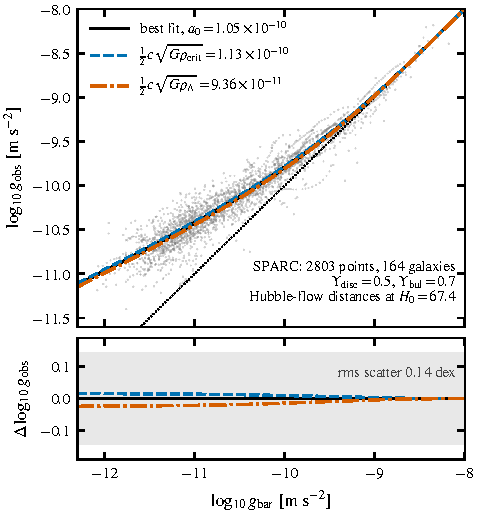
\includegraphics[width=\columnwidth]{fig1_rar.pdf}
\caption{The radial acceleration relation of SPARC (grey points; $\Upsilon_{\rm disc}=0.5$, $\Upsilon_{\rm bul}=0.7$, Hubble-flow distances on $H_0=67.4$) with equation~(\ref{eq:nu}) for three values of $a_0$: the best fit at this mass-to-light ratio (solid), $\tfrac12c\sqrt{G\rho_{\rm crit}}$ (dashed) and $\tfrac12c\sqrt{G\rho_\Lambda}$ (dot-dashed). The dotted line is $g_{\rm obs}=g_{\rm bar}$. Lower panel: the curves relative to the best fit; the band is the rms scatter of the data. The curves differ by less than the scatter everywhere.}
\label{fig:rar}
\end{figure}

\subsection{The standard fit and its degeneracy with the mass-to-light ratio}
\label{sec:standard}
The simplest estimate minimises the residuals in $\log_{10}g_{\rm obs}$ over $a_0$ at fixed mass-to-light ratios. On SPARC's tabulated distances with $\Upsilon_{\rm disc}=0.5$ and $\Upsilon_{\rm bul}=0.7$ we recover the value of \citet{McGaugh2016}, $a_0=1.19\times10^{-10}$ m s$^{-2}$ with an rms scatter of 0.14 dex. On the Planck-consistent distances the same fit gives $1.05\times10^{-10}$ m s$^{-2}$, 12 per cent lower. The result depends steeply on $\Upsilon_{\rm disc}$ (Table~\ref{tab:upsilon}, Fig.~\ref{fig:kappa}a), and equation~(\ref{eq:deep}) shows why. Where stars dominate, $g_{\rm bar}\propto\Upsilon$; in the deep regime the data fix the product $g_{\rm bar}a_0=g_{\rm obs}^2$; so $a_0\propto1/\Upsilon$.

\begin{table}
\caption{The standard fit of equation~(\ref{eq:nu}) to SPARC as a function of the disc mass-to-light ratio ($\Upsilon_{\rm bul}=0.7$; Planck-consistent distances). $\kappa_\Lambda$ and $\kappa_{\rm crit}$ are $a_0$ divided by $c\sqrt{G\rho_\Lambda}$ and by $c\sqrt{G\rho_{\rm crit}}$.}
\label{tab:upsilon}
\begin{tabular}{ccccc}
\toprule
$\Upsilon_{\rm disc}$ & $a_0$ [$10^{-10}$ m s$^{-2}$] & $\kappa_\Lambda$ & $\kappa_{\rm crit}$ & rms [dex]\\
\midrule
0.40 & 1.32 & 0.703 & 0.582 & 0.147\\
0.50 & 1.05 & 0.560 & 0.464 & 0.143\\
0.60 & 0.86 & 0.457 & 0.379 & 0.143\\
0.70 & 0.71 & 0.381 & 0.315 & 0.145\\
0.80 & 0.60 & 0.322 & 0.266 & 0.150\\
\bottomrule
\end{tabular}
\end{table}

The quality of the fit is almost flat across the table, so the data do not choose $\Upsilon_{\rm disc}$. Stellar population models give $\Upsilon_{\rm disc}\simeq0.5$--$0.7$ at 3.6 $\mu$m \citep{Meidt2014,Schombert2019}. In this estimator $\kappa=1/2$ requires $\Upsilon_{\rm disc}=0.555$ for the $\rho_\Lambda$ reading and $0.465$ for the $\rho_{\rm crit}$ reading, the latter just below the population range (on the tabulated distances, 0.621 and 0.524). That is all the standard fit can say. Restricting it to the deep band, $g_{\rm bar}<0.1a_0$, where the stars carry less of the mass, does not remove the dependence: $\kappa=0.50$, $0.44$ and $0.40$ for $\Upsilon_{\rm disc}=0.5$, $0.6$ and $0.7$. (Giving the points whose velocity errors exceed 10 per cent equal weight lowers each value by about 0.1.) Three estimators that depend on the mass-to-light ratio in different ways do better.

\subsection{Estimator A: the Tully--Fisher intercept, with its finite-depth correction}
\label{sec:btfr}
The baryonic Tully--Fisher relation is often quoted as $V_f^4=GM_ba_0$ for the flat rotation velocity $V_f$ and the baryonic mass $M_b$. That is a limit. The exact statement follows from equation~(\ref{eq:nu}) at the outermost measured radius $R$. With $g_{\rm obs}=V_f^2/R=\nu(y)g_{\rm bar}$, write $g_{\rm bar}^2R^2=y\,a_0\times\Gamma GM_b$, where the geometry factor $\Gamma\equiv g_{\rm bar}R^2/(GM_b)$ equals one for a point mass, exceeds one for a disc at finite radius and is read from the SPARC mass model (median 1.19). Then
\begin{equation}
V_f^4=Q(y)\,\Gamma\,GM_ba_0,\qquad Q(y)\equiv\nu^2(y)\,y=1+\sqrt y+\ldots,
\label{eq:btfr}
\end{equation}
so that
\begin{equation}
\hat a_0=\frac{V_f^4}{Q(y)\,\Gamma\,GM_b} .
\label{eq:btfrest}
\end{equation}
The uncorrected ratio $V_f^4/GM_b$ overestimates $a_0$ by the factor $Q\Gamma$. On SPARC this factor is not small. Of the 85 galaxies with flat outer rotation curves, the 24 deepest have outermost accelerations $y<0.05$; for them, on SPARC's tabulated distances, the uncorrected ratio is $1.15\times10^{-10}$ m s$^{-2}$, the typical corrections are $\Gamma\simeq1.19$ and $Q\simeq1.18$, and the corrected, weighted value is $\hat a_0=8.7\times10^{-11}$ m s$^{-2}$ ($\kappa=0.465$). The estimate depends on the Hubble-flow distances through their weight in the sample, 0.20 (our repository's convention audit), so $\hat a_0\propto D_{\rm HF}^{-0.40}$, and on the Planck-consistent convention
\begin{equation}
\kappa_{\rm A}=0.450\pm0.073 .
\label{eq:kappaA}
\end{equation}
The error budget (Table~\ref{tab:budget}) is not dominated by statistics. Its largest term is the form of the transition function. Because of the slow approach in equation~(\ref{eq:deep}), functions that reach the deep regime faster than equation~(\ref{eq:nu}) have $Q$ closer to one and return larger values, up to $\kappa=0.55$. The deepest SPARC galaxy has $y=0.012$; the function would stop mattering only below $y\simeq0.003$.

\begin{table}
\caption{Error budget of estimator A (24 galaxies; effective number 10.1, because five galaxies carry 61 per cent of the weight). Entries are fractional errors on $a_0$ in per cent. The distance-scale term already exceeds the 3.2 per cent shift between SPARC's tabulated distances and the Planck-consistent convention, so the shift is applied to the central value and not added to the error.}
\label{tab:budget}
\begin{tabular}{lr}
\toprule
\emph{random terms} (decrease with sample size) & \\
\quad distances, galaxy by galaxy & 4.8\\
\quad flat velocity & 4.1\\
\quad inclination & 3.9\\
\quad scatter in $\Upsilon$ between galaxies & 3.1\\
\quad H\,{\sc i} fluxes & 1.2\\
\quad \emph{quadrature sum (bootstrap: 8.6)} & 8.1\\
\midrule
\emph{correlated terms} (independent of sample size) & \\
\quad form of the transition function & 8.1\\
\quad zero point of $\Upsilon$ at 3.6 $\mu$m (0.5--0.7) & 6.9\\
\quad H\,{\sc i} flux scale (10 per cent) & 5.9\\
\quad distance scale ($H_0$ and TRGB zero point) & 5.1\\
\quad CO-dark molecular gas (0--10 per cent) & 3.0\\
\quad definition of the flat velocity & 2.2\\
\quad helium correction (1.33--1.40) & 1.5\\
\quad \emph{quadrature sum} & 13.8\\
\midrule
total & 16.2\\
\bottomrule
\end{tabular}
\end{table}

\subsection{A floor that no sample removes}
\label{sec:floor}
Two of the correlated terms cannot be reduced by choosing the sample. The baryonic mass is $M_b=\Upsilon L+M_{\rm gas}$. Let $f_*$ be the stellar fraction of $M_b$, $s_\Upsilon$ the fractional uncertainty of the stellar mass scale and $s_g$ that of the gas mass scale. The fractional error on $M_b$, and so on $a_0$ in equation~(\ref{eq:btfrest}), is
\begin{equation}
\sigma(f_*)=\sqrt{(f_*s_\Upsilon)^2+\big[(1-f_*)s_g\big]^2} .
\end{equation}
Choosing gas-rich galaxies lowers $f_*$ and suppresses the first term, but it hands the budget to the second. The minimum follows from $d\sigma^2/df_*=0$:
\begin{equation}
f_*=\frac{s_g^2}{s_\Upsilon^2+s_g^2},\qquad
\sigma_{\min}=\frac{s_\Upsilon s_g}{\sqrt{s_\Upsilon^2+s_g^2}} .
\label{eq:floor}
\end{equation}
With $s_\Upsilon=0.17$ (the range $0.5$--$0.7$ about $0.6$) and $s_g=0.115$ (H\,{\sc i} flux scale, helium and CO-dark gas in quadrature) the floor is $\sigma_{\min}=9.5$ per cent, reached at $f_*=0.32$. It does not depend on the number of galaxies, on the transition function, or on distances. Even if both scales were known to 5 per cent the floor would be 3.5 per cent. The route to a better $\kappa$ therefore runs through the calibration of stellar and gas masses, not through larger samples.

\subsection{Estimator B: the shape of the relation, immune to a common distance scale}
\label{sec:shape}
Suppose all distances are wrong by a common factor. In the plane of Fig.~\ref{fig:rar} that is a purely vertical shift, because $g_{\rm bar}$ does not change and $g_{\rm obs}\propto1/D$. We therefore fit
\begin{equation}
\log_{10}g_{\rm obs}=\log_{10}\!\big[g_{\rm bar}\,\nu(g_{\rm bar}/a_0)\big]+C
\end{equation}
with the offset $C$ free. The offset absorbs the distance scale, and $a_0$ is fixed by where the bend lies along the $g_{\rm bar}$ axis. On SPARC, rescaling every distance by 5 or 10 per cent changes this $a_0$ by less than one part in $10^{10}$, while the standard fit moves by 22 per cent for a 10 per cent rescaling.

The price of the immunity is a strong dependence on the mass-to-light ratios, above all that of the bulges, because the bend is located using the high-acceleration points where bulges dominate. Table~\ref{tab:shape} gives the result over the ranges $\Upsilon_{\rm disc}=0.5$--$0.7$ and $\Upsilon_{\rm bul}=0.6$--$0.8$. At the centre of the grid $\kappa=0.584$. The half-range over the grid is 0.146, of which the bulge term alone is 0.124 and the disc term 0.022. An 11.5 per cent change of the gas scale moves $\kappa$ by 0.048, and a bootstrap over galaxies gives a statistical error of 0.102, far larger than the formal error of the fit, because a few bulge-dominated galaxies carry the high-acceleration end. In quadrature,
\begin{equation}
\kappa_{\rm B}=0.58\pm0.18 .
\label{eq:kappaB}
\end{equation}
\ifpapersix An earlier version of this estimator held $\Upsilon_{\rm bul}$ fixed, used the formal statistical error and SPARC's tabulated distances, which gave $0.551\pm0.043$ \citep{Zimmerman2026kappa}; that error bar was too small by a factor of four. (The four-form section of that note is superseded.) \else An earlier version of this estimator held $\Upsilon_{\rm bul}$ fixed and used the formal statistical error and SPARC's tabulated distances, which gave $0.551\pm0.043$; that error bar was too small by a factor of four. \fi Restricting the fit to the 132 galaxies without bulges does not help. Their baryonic accelerations stop at $16a_0$, the lever arm is too short to locate the bend, and $\kappa$ runs from 0.51 to 1.13 across $\Upsilon_{\rm disc}=0.5$--$0.7$. The immunity is also to a \emph{common} rescaling only. The Hubble-flow galaxies lie preferentially at the high-acceleration end of the relation, where the estimator locates the bend, so the $H_0$ convention moves it: from 0.584 (Planck-consistent) to 0.547 on the tabulated distances and to 0.489--0.505 with $\rho_\Lambda$ rebuilt at $H_0=73$ (Table~\ref{tab:conv}). Estimator B is therefore a cross-check on the distance scale and a poor measurement of $\kappa$.

\begin{table}
\caption{Estimator B (shape-only; Planck-consistent distances): $\kappa$ as a function of the two stellar mass-to-light ratios.}
\label{tab:shape}
\begin{tabular}{lccc}
\toprule
 & $\Upsilon_{\rm bul}=0.6$ & $0.7$ & $0.8$\\
\midrule
$\Upsilon_{\rm disc}=0.5$ & 0.444 & 0.567 & 0.715\\
$\Upsilon_{\rm disc}=0.6$ & 0.470 & 0.584 & 0.718\\
$\Upsilon_{\rm disc}=0.7$ & 0.502 & 0.610 & 0.735\\
\bottomrule
\end{tabular}
\end{table}

\subsection{Estimator C: a profile likelihood with the mass-to-light ratio free for every galaxy}
\label{sec:profile}
The degeneracy between $\Upsilon$ and $a_0$ is exact in the deep regime only if every baryonic component scales with $\Upsilon$. The gas does not, and the transition region does not, so freeing the stellar mass-to-light ratio galaxy by galaxy still leaves $a_0$ constrained. We profile the likelihood of equation~(\ref{eq:nu}) over all SPARC points ($V>0$, velocity errors clipped at 1 km s$^{-1}$), with $\Upsilon_{\rm disc}$ free for each galaxy, $\Upsilon_{\rm bul}=1.4\,\Upsilon_{\rm disc}$, the gas fixed, and an intrinsic scatter (0.077 dex) set by $\chi^2/{\rm d.o.f.}=1$ at the best fit. Unlike the ratios of the pitfall in Section~\ref{sec:deepregime}, these are fitted jointly with $a_0$. On the Planck-consistent distances the best fit for 175 galaxies (3391 points) is $a_0=8.1\times10^{-11}$ m s$^{-2}$, with a galaxy bootstrap error of 9.3 per cent. Two systematic terms dominate. An 11.5 per cent change of the gas scale, to which an estimate anchored by the gas is directly exposed, moves $\kappa$ by 0.039. And the transition function matters: the same likelihood with $g_{\rm obs}^2=g_{\rm bar}^2+g_{\rm bar}a_0$ gives $\kappa=0.54$, so half the difference, 0.053, is carried as a term. In quadrature,
\begin{equation}
\kappa_{\rm C}=0.43\pm0.08 .
\label{eq:kappaC}
\end{equation}
An earlier analysis in our repository used the second function and SPARC's tabulated distances and found $a_0=1.08\times10^{-10}$ m s$^{-2}$ ($\kappa_\Lambda=0.575$); our code reproduces that result exactly when given its inputs, and the difference from equation~(\ref{eq:kappaC}) is the two choices just named.

\subsection{Do the estimators measure, or echo an assumed value?}
\label{sec:injection}
Every estimator above contains $a_0$ somewhere in its machinery, so we test them on synthetic data. We keep the real SPARC baryons, generate $g_{\rm obs}$ from equation~(\ref{eq:nu}) with a known $a_0$ equal to 0.7, 1.0 and 1.3 times the value of equation~(\ref{eq:a0value}), and add the quoted velocity errors plus 0.034 dex of intrinsic scatter. The standard fit returns the injected value to within 1 per cent and the deep-band fit to within 2.1 per cent. The shape-only fit returns it to within 2.3 per cent even when every $g_{\rm obs}$ is shifted by a common 0.08 dex, the effect of a 20 per cent distance error, which moves the standard fit by 60 to 66 per cent. Estimator A evaluates its correction $Q(y)$ at an assumed $a_0$; this is a sensitivity test on the real data rather than an injection. Iterating the correction to the estimator's own output changes the result by 0.6 per cent, and raising the assumed value by 21 per cent changes it by 9 per cent. None of the measured values is an echo of an assumed one.

\subsection{The deep regime in two surveys: slope and amplitude}
\label{sec:deepregime}
Below $a_0$ equation~(\ref{eq:nu}) predicts two things: how steeply $g_{\rm obs}$ rises with $g_{\rm bar}$, and where the curve lies. With $n(y)\equiv{\rm d}\ln\nu/{\rm d}\ln y$,
\begin{equation}
\beta(y)\equiv\frac{{\rm d}\ln g_{\rm obs}}{{\rm d}\ln g_{\rm bar}}=1+n(y)=1-\frac{\sqrt y/2}{e^{\sqrt y}-1}=\frac12+\frac{\sqrt y}{4}+\ldots
\label{eq:beta}
\end{equation}
The slope tends to one half and approaches it just as slowly: $\beta=0.525$, $0.554$, $0.575$ and $0.603$ at $y=0.01$, $0.05$, $0.1$ and $0.2$. A measured deep slope must therefore be compared with equation~(\ref{eq:beta}) at the accelerations actually sampled, not with one half. Moving $a_0$ from the $\rho_\Lambda$ value to the $\rho_{\rm crit}$ value changes the expected slope at the SPARC points by less than 0.01, so the slope tests the form of the relation and the amplitude tests $\kappa$.

We use the window $g_{\rm bar}<0.2a_0=1.87\times10^{-11}$ m s$^{-2}$, with $a_0$ fixed at the value of equation~(\ref{eq:a0value}), in two surveys with independent data and mass models. The first is SPARC, as above. The second is MIGHTEE-HI \citep{Varasteanu2025}: 19 H\,{\sc i}-selected galaxies at $z<0.08$ with MeerKAT rotation curves and stellar masses from resolved fits to their spectral energy distributions (SED). The survey publishes its radial acceleration relation only as a figure. We digitised its 80 points from the vector graphics; fitting equation~(\ref{eq:nu}) to them returns the survey's own value of $a_0$ to 1.2 per cent. We identify galaxies by marker colour, which is not a clean identifier: the figure has 18 colours for 19 galaxies, and the largest group, 11 points spanning only 0.22 dex in $g_{\rm bar}$, may hold two. The window holds 72 of the points, 70 of them in the 17 groups with at least three.

\emph{The slope.} For each galaxy with at least three points in the window we fit a straight line to $\log g_{\rm obs}$ against $\log g_{\rm bar}$, and we take the median over galaxies. Offsets that are constant within a galaxy, from its distance, its inclination or its stellar mass-to-light ratio, do not bias this statistic, so it does not depend on the $H_0$ convention. The expectation is the same statistic computed from $g_{\rm bar}\nu(g_{\rm bar}/a_0)$ at the same points, and a bootstrap over galaxies gives the error of the difference. Table~\ref{tab:deep} and Fig.~\ref{fig:deep}(a) show the result. SPARC gives $\beta=0.58$--$0.62$ against an expectation of 0.57, and MIGHTEE-HI gives $0.60\pm0.08$ against 0.56 ($0.60\pm0.09$ against 0.56 without the largest colour group); the differences lie between 0.1 and $1.6\sigma$. Together the two surveys exclude a slope of 0.75 at 4.2--$4.9\sigma$ and the Newtonian slope at $12\sigma$. On synthetic data built on the real baryons the statistic is unbiased to 0.005, and it returns an injected slope of 0.75 as 0.751 (SPARC) and 0.752 (MIGHTEE-HI). A single straight line through all the SPARC points in the window, which is exposed to the galaxy-to-galaxy offsets, also agrees: 0.52--0.57 against 0.56. The survey's own fit finds a low-acceleration slope near one half \citep{Varasteanu2025}.

\emph{The amplitude.} Fitting equation~(\ref{eq:nu}) in the window gives, on SPARC, $\kappa_\Lambda=0.54\pm0.04$, $0.47\pm0.03$ and $0.41\pm0.03$ for $\Upsilon_{\rm disc}=0.5$, 0.6 and 0.7 (bootstrap over galaxies), a range that contains one half. MIGHTEE-HI gives $\kappa_\Lambda=0.89\pm0.13$, and the survey's own fit to all radii gives $0.90\pm0.07$. Taken at face value, the survey's own value and SPARC disagree by 5.0 to $7.5\sigma$ in $\ln a_0$. The disagreement lies mostly in the stellar mass-to-light ratio. The SED fits of MIGHTEE-HI have a median of 0.35 in the $K_s$ band, whereas another recent determination in the same band finds a median of 0.72 \citep{Marasco2025}. When the survey fixes $\Upsilon_K=0.6$ it obtains $a_0=(1.08\pm0.09)\times10^{-10}$ m s$^{-2}$, that is $\kappa_\Lambda=0.58\pm0.05$, which lies 0.7 and $2.0\sigma$ above SPARC at $\Upsilon_{\rm disc}=0.5$ and 0.6 but $3.1\sigma$ above it at 0.7 (Fig.~\ref{fig:deep}b; the comparison also carries any difference between the two surveys' distance conventions). The deep regime therefore agrees with $\kappa\simeq1/2$ when the two surveys use comparable mass-to-light ratios, its amplitude is set by that choice rather than by the relation, and it cannot separate the $\rho_\Lambda$ reading from the $\rho_{\rm crit}$ reading.

\emph{A pitfall.} The amplitude is only as good as the stellar masses. Mass-to-light ratios fitted galaxy by galaxy to the rotation curves without the relation absorb part of the mass discrepancy into the stars: in one such compilation of SPARC disc ratios (median 1.17, up to 15) their logarithms correlate at $r=0.92$ with those of the ratio at which the baryons alone reproduce each curve. Used in the window fit, they give $\kappa_\Lambda=0.25\pm0.03$, a factor of 1.7 to 2.2 below the population ratios, and they manufacture an apparent deficit in the deep regime.

\begin{table}
\caption{The deep regime, $g_{\rm bar}<0.2a_0$. $\beta$ is the median over galaxies of the slope of $\log g_{\rm obs}$ against $\log g_{\rm bar}$; $\beta_\nu$ is the same statistic computed from equation~(\ref{eq:nu}) at the same points, with $\kappa_\Lambda=1/2$; $\Delta/\sigma$ is their difference in units of its bootstrap error. $\kappa_\Lambda$ is equation~(\ref{eq:nu}) fitted in the window (SPARC on the Planck-consistent distances), except in the rows marked V25, which are the fits of \citet{Varasteanu2025} to all radii under their stated mass-to-light conventions. The last row uses mass-to-light ratios fitted to the rotation curves themselves (Section~\ref{sec:deepregime}).}
\label{tab:deep}
\setlength{\tabcolsep}{3.5pt}
\begin{tabular}{@{}lccccc@{}}
\toprule
sample & $N_{\rm gal}$ & $\beta$ & $\beta_\nu$ & $\Delta/\sigma$ & $\kappa_\Lambda$\\
\midrule
SPARC, $\Upsilon_{\rm disc}=0.5$ & 125 & $0.62\pm0.03$ & 0.570 & $+1.6$ & $0.54\pm0.04$\\
SPARC, $\Upsilon_{\rm disc}=0.6$ & 120 & $0.61\pm0.03$ & 0.573 & $+1.3$ & $0.47\pm0.03$\\
SPARC, $\Upsilon_{\rm disc}=0.7$ & 116 & $0.58\pm0.04$ & 0.575 & $+0.1$ & $0.41\pm0.03$\\
MIGHTEE-HI, digitised & 17 & $0.60\pm0.08$ & 0.556 & $+0.5$ & $0.89\pm0.13$\\
\midrule
V25, SED ratios & 19 & & & & $0.90\pm0.07$\\
V25, no H$_2$ & 19 & & & & $1.10\pm0.08$\\
V25, radial mean & 19 & & & & $0.79\pm0.07$\\
V25, $\Upsilon_K=0.6$ & 19 & & & & $0.58\pm0.05$\\
\midrule
SPARC, fitted ratios & & & & & $0.25\pm0.03$\\
\bottomrule
\end{tabular}
\end{table}

\subsection{What the measurements say}
\label{sec:measure}
Table~\ref{tab:cands} and Fig.~\ref{fig:kappa}(b) compare the three estimators with the candidate coefficients, and Table~\ref{tab:conv} gives each on four $H_0$ conventions. On the Planck-consistent convention $\kappa=1/2$ lies $0.7\sigma$ from estimator A, $0.5\sigma$ from B and $0.9\sigma$ from C. The coincidence $cH_\Lambda/2\pi$ does as well, and on a common footing Milgrom's $2\pi$ forms are at least as close to A and C as $1/2$ is: $cH_\Lambda/2\pi$ against $1/2$ on the $\rho_\Lambda$ footing, and $cH_0/2\pi$ ($1.5$ and $1.6\sigma$) against $\tfrac12c\sqrt{G\rho_{\rm crit}}$ ($2.1$ and $2.2\sigma$) on the critical density. The estimators share galaxies and calibrations, so we neither average them nor multiply their likelihoods. Taken one at a time, the likelihood ratio between $\kappa=1/2$ and $0.461$ is $e^{-0.22}$ (A), $e^{+0.12}$ (B) and $e^{-0.31}$ (C): the data do not distinguish them. The thermal identifications are excluded: $a_0=cH_\Lambda$ by a factor of six and the $2cH_\Lambda$ of \citet{Milgrom1999} by a factor of 12.

Published determinations, converted in Table~\ref{tab:pub}, show that the inferred coefficient follows the treatment of the stellar mass-to-light ratio. Against our working value: the full joint inference of \citet{Desmond2023} over distances, inclinations, luminosities and mass-to-light ratios finds $a_0=(1.19\pm0.04\pm0.09)\times10^{-10}$ m s$^{-2}$, which is $\kappa_\Lambda=0.636\pm0.053$; it puts $\kappa=1/2$ at $2.6\sigma$ on the $\rho_\Lambda$ footing (and 0.461 at $3.3\sigma$), and $\tfrac12c\sqrt{G\rho_{\rm crit}}$ at $0.6\sigma$ (and $cH_0/2\pi$ at $1.5\sigma$) on the critical density. That inference, like \citet{McGaugh2016}, starts from SPARC's tabulated distances, on which our standard fit is 12 per cent higher than on the Planck-consistent convention; we do not convert it, because its distances are free parameters with priors. The MIGHTEE-HI determinations of \citet{Varasteanu2025,Varasteanu2026}, $\kappa_\Lambda=0.80$--$0.90$ with their SED-based ratios and $0.58$ with $\Upsilon_K=0.6$, make the same point in an independent survey.

We adopt $\kappa=1/2$ as the working value because it is the simplest number consistent with our three estimators, and for no deeper reason: it is fitted, and a published joint inference disfavours it at $2.6\sigma$ on its own footing. Separating it from $0.461$ at $3\sigma$ would need $a_0$ to 2.6 per cent, below the floor of equation~(\ref{eq:floor}). The deep regime of Section~\ref{sec:deepregime} is a consistency test rather than a fourth estimator, because its amplitude follows the stellar mass-to-light convention.

\begin{table}
\caption{Candidate coefficients in $a_0=\kappa c\sqrt{G\rho_\Lambda}$ and their distance, in standard deviations, from estimators A ($0.450\pm0.073$), B ($0.58\pm0.18$) and C ($0.43\pm0.08$), all on the Planck-consistent convention. The last row is $\kappa=1/2$ on the critical density, expressed as $\kappa_\Lambda$.}
\label{tab:cands}
\setlength{\tabcolsep}{3.5pt}
\begin{tabular}{@{}lcccc@{}}
\toprule
$a_0$ & $\kappa$ & A & B & C\\
\midrule
$cH_\Lambda/2\pi$ \citep{Milgrom2020} & 0.461 & $+0.1$ & $-0.7$ & $+0.4$ \\
$\tfrac12c\sqrt{G\rho_\Lambda}$ (working value) & 0.500 & $+0.7$ & $-0.5$ & $+0.9$ \\
$cH_0/2\pi$ \citep{Milgrom2020} & 0.557 & $+1.5$ & $-0.1$ & $+1.6$ \\
$cH_0/6$ \citep{Verlinde2017} & 0.583 & $+1.8$ & $0.0$ & $+1.9$ \\
$cH_\Lambda$ (Unruh $=$ de Sitter temperature) & 2.89 & $+33$ & $+13$ & $+32$ \\
$2cH_\Lambda$ \citep{Milgrom1999} & 5.79 & $+73$ & $+28$ & $+70$ \\
\midrule
$\tfrac12c\sqrt{G\rho_{\rm crit}}$ & 0.604 & $+2.1$ & $+0.1$ & $+2.2$ \\
\bottomrule
\end{tabular}
\end{table}

\begin{table}
\caption{The three estimators of $\kappa_\Lambda$ on four $H_0$ conventions. Planck-consistent (adopted): SPARC's Hubble-flow distances moved to $H_0=67.4$. Tabulated: SPARC's distances as published (Hubble flow at 73) with $\rho_\Lambda$ at 67.4. R2a and R2b: SPARC's distances with $\rho_\Lambda$ rebuilt at $H_0=73$, holding $\Omega_\Lambda$ or $\Omega_mh^2$ fixed. The conventions are alternatives, not errors.}
\label{tab:conv}
\setlength{\tabcolsep}{3.5pt}
\begin{tabular}{@{}lcccc@{}}
\toprule
estimator & Planck-consistent & tabulated & R2a & R2b\\
\midrule
A: Tully--Fisher intercept & 0.450 & 0.465 & 0.429 & 0.416 \\
B: shape only & 0.584 & 0.547 & 0.505 & 0.489 \\
C: profile likelihood & 0.434 & 0.469 & 0.433 & 0.419 \\
\bottomrule
\end{tabular}
\end{table}

\begin{table*}
\caption{Determinations of $a_0$ converted to $\kappa$ on the two footings, with each analysis's treatment of the stellar mass-to-light ratio. Published values are converted as published (their own distance conventions); errors combine statistical and systematic terms in quadrature where both are given. This paper's values are on the Planck-consistent convention.}
\label{tab:pub}
\begin{tabular}{llllcc}
\toprule
analysis & sample & mass-to-light ratio & $a_0$ [$10^{-10}$ m s$^{-2}$] & $\kappa_\Lambda$ & $\kappa_{\rm crit}$\\
\midrule
\citet{McGaugh2016} & SPARC & fixed: 0.5 / 0.7 & $1.20\pm0.24$ & $0.64\pm0.13$ & $0.53\pm0.11$ \\
\citet{Desmond2023} & SPARC & free (joint inference) & $1.19\pm0.10$ & $0.64\pm0.05$ & $0.53\pm0.04$ \\
\citet{Varasteanu2025} & MIGHTEE-HI & resolved SED fits & $1.69\pm0.13$ & $0.90\pm0.07$ & $0.75\pm0.06$ \\
\citet{Varasteanu2025} & MIGHTEE-HI & $\Upsilon_K=0.6$ fixed & $1.08\pm0.09$ & $0.58\pm0.05$ & $0.48\pm0.04$ \\
\citet{Varasteanu2026} & MIGHTEE-HI/LADUMA & fiducial (varying) & $1.50\pm0.05$ & $0.80\pm0.03$ & $0.66\pm0.02$ \\
this paper, estimator A & SPARC & 0.5--0.7 (budget) & $0.84\pm0.14$ & $0.45\pm0.07$ & $0.37\pm0.06$ \\
this paper, estimator B & SPARC & grid, Table~\ref{tab:shape} & $1.09\pm0.35$ & $0.58\pm0.18$ & $0.48\pm0.15$ \\
this paper, estimator C & SPARC & free per galaxy & $0.81\pm0.14$ & $0.43\pm0.08$ & $0.36\pm0.06$ \\
\bottomrule
\end{tabular}
\end{table*}

\begin{figure*}
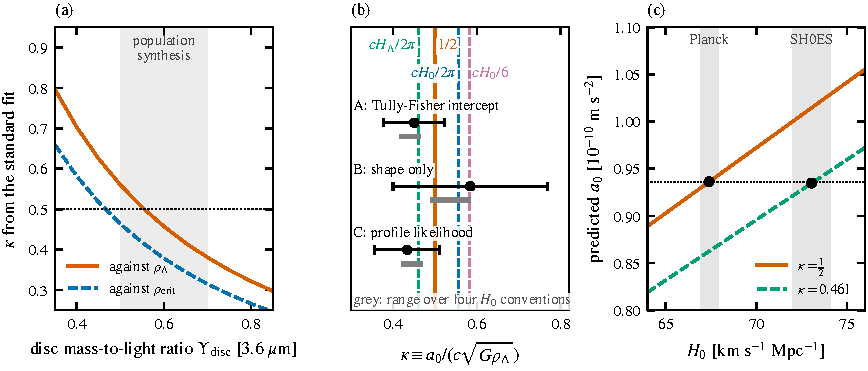
\includegraphics[width=\textwidth]{fig2_kappa.pdf}
\caption{(a) The coefficient returned by the standard fit as a function of the disc mass-to-light ratio, measured against $\rho_\Lambda$ (solid) and against $\rho_{\rm crit}$ (dashed), on the Planck-consistent distances; the band is the range of stellar population models. (b) Estimators A, B and C (points with $1\sigma$ total errors, Planck-consistent convention) against the candidate coefficients of Table~\ref{tab:cands}. Grey bars: the full range of each estimator over the four $H_0$ conventions of Table~\ref{tab:conv}, computed by the same scripts; they are alternatives rather than errors, so they need not be symmetric about the point. (c) The $H_0$ lock: the $a_0$ predicted by $\kappa=1/2$ (solid) and by $\kappa=0.461$ (dashed) as a function of $H_0$ at fixed $\Omega_\Lambda$. The two black points, at the Planck and SH0ES values of $H_0$, coincide to 0.2 per cent.}
\label{fig:kappa}
\end{figure*}

\begin{figure*}
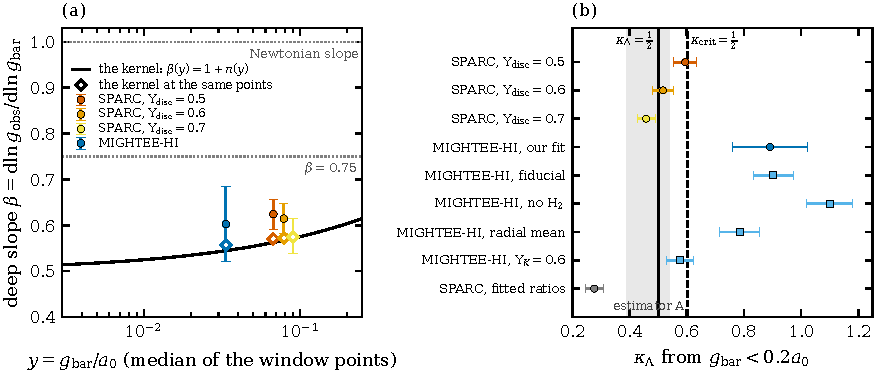
\includegraphics[width=\textwidth]{fig_deep.pdf}
\caption{The deep regime in two surveys. (a) The slope of the relation. The curve is equation~(\ref{eq:beta}). Filled points are the median per-galaxy slopes of SPARC, at three disc mass-to-light ratios, and of MIGHTEE-HI in the window $g_{\rm bar}<0.2a_0$, placed at the median $y$ of their points (the SPARC points are offset by $\pm10$ per cent for clarity), with bootstrap errors. Open diamonds are the same statistic computed from equation~(\ref{eq:nu}) at the same points. The dotted lines mark a slope of 0.75 and the Newtonian slope. (b) The coefficient in the deep regime: SPARC at three disc ratios (Planck-consistent distances) and our fit to the digitised MIGHTEE-HI points, both in the window (circles); the survey's own fits to all radii under four mass-to-light conventions (squares); and SPARC in the window with mass-to-light ratios fitted to the rotation curves themselves (grey). The solid and dashed lines are $\kappa=1/2$ against $\rho_\Lambda$ and against $\rho_{\rm crit}$; the grey band is estimator A.}
\label{fig:deep}
\end{figure*}

\subsection{The coefficient is degenerate with the Hubble constant}
\label{sec:h0}
Substituting $\rho_{\rm crit}$ into equation~(\ref{eq:relation}) gives $a_0=\kappa\,cH_0\sqrt{3\Omega_\Lambda/8\pi}$: at fixed $\Omega_\Lambda$ the predicted acceleration depends only on the product $\kappa H_0$. The two values of the Hubble constant currently in tension, $67.4$ \citep{Planck2020} and $73.04$ km s$^{-1}$ Mpc$^{-1}$ \citep{Riess2022}, have the ratio $0.923$, and $0.461/0.500=0.921$, so $(\kappa,H_0)=(0.500,67.4)$ and $(0.461,73.04)$ predict the same $a_0$ to 0.2 per cent (Fig.~\ref{fig:kappa}c); with $\Omega_mh^2$ held at its CMB value instead, the matching coefficient is 0.446. The first statement is exact; the second is a numerical coincidence to which we attach no meaning. A claim that the coefficient is `exactly one half' is also a claim about $H_0$ and about the distance scale of the galaxies, which is why Section~\ref{sec:data} fixes the convention. Read in reverse at $\kappa=1/2$, with the Hubble-flow distances rebuilt at each trial $H_0$, estimator A gives $H_0=57\pm15$ and estimator B $73\pm15$ km s$^{-1}$ Mpc$^{-1}$ (their sensitivities to those distances have opposite signs), far too coarse to bear on the tension.

%=====================================================================================================================
\section{The redshift test}
\label{sec:ztest}
The value of $\kappa$ cannot distinguish $\rho_\Lambda$ from $\rho_{\rm crit}$, nor either from an emergent scale. The redshift dependence can. We define
\begin{equation}
\Delta(z)\equiv\log_{10}\frac{a_0(z)}{a_0(0)} .
\end{equation}

\subsection{Three laws}
\label{sec:laws}
\emph{(a) A scale anchored to $\Lambda$.} The cosmological constant does not evolve, so $\rho_\Lambda$ and $a_0$ are the same at every redshift:
\begin{equation}
\Delta_\Lambda(z)=0 .
\label{eq:lawflat}
\end{equation}
This is the content of the hypothesis, not evidence for it. Plain MOND, in which $a_0$ is simply a constant of nature, makes the same prediction. What the $\Lambda$ anchor adds is a reason for the constancy, and with it the exclusion of law (b).

\emph{(b) A scale anchored to the critical density.} Replacing $\rho_\Lambda$ by $\rho_{\rm crit}(z)=3H^2(z)/8\pi G$ gives $a_0\propto H(z)$. With $E(z)\equiv H(z)/H_0=[\Omega_m(1+z)^3+\Omega_\Lambda]^{1/2}$,
\begin{equation}
\Delta_H(z)=\log_{10}E(z) .
\label{eq:lawH}
\end{equation}
At $z=2.5$, $E^2=0.315\times3.5^3+0.685=14.19$, so $E=3.77$ and $\Delta_H=+0.58$. At $z=1.2$, the limit of \citet{Limbach2008}, it is $+0.30$; at $z=2$ the factor is 3.0, below the factor of about four that \citet{Milgrom2017} considers all but excluded by the \citet{Genzel2017} discs.

\emph{(c) The emergent scale of $\Lambda$CDM haloes.} In $\Lambda$CDM the characteristic acceleration of the relation is inherited from dark-matter haloes. Appendix~\ref{app:nfw} shows that the central acceleration of an NFW halo \citep{NFW1997} of mass $M_{200}$ and concentration $c_{200}$ is
\begin{equation}
g_{\max}=\frac{100^{2/3}}{2}\,(GM_{200})^{1/3}H^{4/3}(z)\,\frac{c_{200}^2}{f(c_{200})},
\label{eq:gmax}
\end{equation}
where $f(x)=\ln(1+x)-x/(1+x)$. For $M_{200}=10^{12}\,{\rm M_\odot}$ today this is $8.1\times10^{-11}$ m s$^{-2}$, close to $a_0$, which is part of the reason that galaxies in $\Lambda$CDM haloes show an $a_0$-like scale \citep{Navarro2017}. At fixed halo mass,
\begin{equation}
\Delta_{\rm halo}(z)=\tfrac43\log_{10}E(z)+\log_{10}\frac{[c^2/f(c)]_z}{[c^2/f(c)]_0} .
\label{eq:lawhalo}
\end{equation}
The first term rises, because haloes of a given mass were denser in the past. The second falls, because they were less concentrated. With the concentration--mass relation of \citet{DuttonMaccio2014}, $c_{200}$ of a $10^{12}\,{\rm M_\odot}$ halo falls from 8.4 to 3.9 between $z=0$ and $2.5$, and $\Delta_{\rm halo}(2.5)=0.768-0.440=+0.33$, a factor 2.13. That number should not be used as the decision value, because it depends on the halo mass: over $M_{200}=10^{11}$--$10^{13}\,{\rm M_\odot}$ and the relations of \citet{DuttonMaccio2014} and \citet{Duffy2008} it runs from $+0.23$ to $+0.46$ (Table~\ref{tab:laws}). The halo mass that matters is the one the measurement selects. The gate of Section~\ref{sec:design} admits discs with $V_f\simeq83$--$125$ km s$^{-1}$; at $z=2.5$, for $V_f/V_{200}=1.0$--$1.2$, their haloes have $M_{200}=3\times10^{10}$--$1.8\times10^{11}\,{\rm M_\odot}$, where the Dutton--Macci\`o relation gives $+0.17$ to $+0.25$ dex. We adopt the value for the central example ($M_{200}=7.9\times10^{10}\,{\rm M_\odot}$),
\begin{equation}
\Delta_{\rm halo}(2.5)=+0.22 ,
\label{eq:dgate}
\end{equation}
as the decision value. The choice of concentration--mass relation is a model systematic of the same size: \citet{Duffy2008} give $+0.43$ for the same haloes. A different structural scaling, the Tully--Fisher ratio $V_{\max}^4/GM$ at a fixed ratio of baryonic to halo mass, gives $+0.56$ for $10^{12}\,{\rm M_\odot}$ (Appendix~\ref{app:nfw}). Hydrodynamical simulations point the same way: \citet{KellerWadsley2017} find that the simulated relation is not constant with redshift, and in the Magneticum simulations the best-fitting $a_0$ rises by a factor of about three between $z=0$ and 2 \citep{Mayer2023}, which is $+0.48$ dex. Every $\Lambda$CDM estimate is a rise of 0.17--0.6 dex at $z=2.5$. The $g_{\max}$ proxy is itself a heuristic, not a $\Lambda$CDM prediction for the statistic of the decision rule; calibrating the $\Lambda$CDM side on simulated low-mass discs inverted in the same way at $y<0.3$ would replace it and is not done here. Section~\ref{sec:design} carries the relation spread as a systematic of the design.

\emph{(d) If dark energy evolves.} Law (a) assumes a true cosmological constant. If instead $a_0$ followed an evolving dark-energy density, $a_0\propto\sqrt{\rho_{\rm DE}(z)}$, then for the $w_0w_a$ fits of \citet{DESI2025}
\begin{equation}
\frac{\rho_{\rm DE}(z)}{\rho_{\rm DE}(0)}=(1+z)^{3(1+w_0+w_a)}\exp\!\Big[-\frac{3w_az}{1+z}\Big]
\end{equation}
gives $\Delta=-0.09$ to $-0.11$ at $z=2.5$ for the three supernova combinations. This is not our prediction. We quote it to show that the test is robust to the question: the alternatives to constancy differ from it by $+0.2$ to $+0.6$ dex, while this differs by $-0.1$.

\begin{table}
\caption{$\Delta(z)=\log_{10}[a_0(z)/a_0(0)]$ in dex for the laws of Section~\ref{sec:laws}. Column 4: the halo law for $M_{200}=10^{12}\,{\rm M_\odot}$ with the concentrations of \citet{DuttonMaccio2014} (used for the massive discs of Section~\ref{sec:existing}); column 5: the range over $10^{11}$--$10^{13}\,{\rm M_\odot}$ and the relations of \citet{DuttonMaccio2014} and \citet{Duffy2008}; column 6: the halo law for the gate's central disc ($V_f=105$ km s$^{-1}$, $V_f/V_{200}=1.1$), whose halo mass is set at each redshift. The last column is the density mapping of Section~\ref{sec:laws}(d) for the DESI+CMB+DESY5 fit.}
\label{tab:laws}
\setlength{\tabcolsep}{4pt}
\begin{tabular}{@{}ccccccc@{}}
\toprule
$z$ & $\Lambda$ & $H(z)$ & halo & halo, range & halo, gate & $\sqrt{\rho_{\rm DE}}$\\
\midrule
1.0 & 0 & $+0.25$ & $+0.09$ & $[+0.05,+0.16]$ & $+0.06$ & $+0.00$\\
2.0 & 0 & $+0.48$ & $+0.25$ & $[+0.16,+0.37]$ & $+0.16$ & $-0.07$\\
2.5 & 0 & $+0.58$ & $+0.33$ & $[+0.23,+0.46]$ & $+0.22$ & $-0.10$\\
3.0 & 0 & $+0.66$ & $+0.41$ & $[+0.29,+0.54]$ & $+0.27$ & $-0.13$\\
\bottomrule
\end{tabular}
\end{table}

\begin{figure}
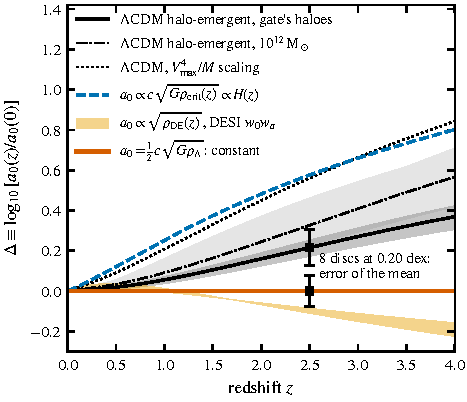
\includegraphics[width=\columnwidth]{fig3_laws.pdf}
\caption{$\Delta(z)$ for the laws of Section~\ref{sec:laws}: a scale anchored to $\Lambda$ (thick horizontal line), a scale anchored to the critical density (dashed), and the $\Lambda$CDM halo-emergent scale for the haloes selected by the gate of Section~\ref{sec:design} (solid black; dark band: the gate's examples and $V_f/V_{200}=1.0$--$1.2$), for $10^{12}\,{\rm M_\odot}$ (dot-dashed), and its range over halo mass and concentration--mass relation (light band); dotted: the $V_{\max}^4/M$ scaling. The narrow shaded band is the density mapping under the DESI DR2 $w_0w_a$ fits, shown for scale. The two squares at $z=2.5$ mark the decision values $0$ and $+0.22$, with error bars equal to the standard error of the sample mean of the recommended design (eight galaxies at 0.20 dex) under each hypothesis.}
\label{fig:laws}
\end{figure}

\subsection{The statistic, and why the depth of the galaxy matters}
\label{sec:amp}
Given $g_{\rm obs}$ and $g_{\rm bar}$ at one radius of one galaxy, equation~(\ref{eq:nu}) can be solved for $a_0$ exactly: find the $y$ for which $\nu(y)=g_{\rm obs}/g_{\rm bar}$ and set
\begin{equation}
\hat a_0=\frac{g_{\rm bar}}{y} .
\label{eq:invert}
\end{equation}
Unlike the deep-regime formula $g_{\rm obs}^2/g_{\rm bar}$, this is unbiased at any acceleration. Its precision is another matter. Taking the logarithm of $\nu(y)=g_{\rm obs}/g_{\rm bar}$ and differentiating, with $n\equiv d\ln\nu/d\ln y$, gives $n\,d\ln y=d\ln g_{\rm obs}-d\ln g_{\rm bar}$; since $d\ln\hat a_0=d\ln g_{\rm bar}-d\ln y$,
\begin{equation}
d\ln\hat a_0=-\frac1n\,d\ln g_{\rm obs}+\Big(1+\frac1n\Big)d\ln g_{\rm bar},\qquad n=-\frac{\sqrt y/2}{e^{\sqrt y}-1} .
\label{eq:amp}
\end{equation}
Errors in the kinematics are therefore multiplied by $A_{\rm obs}=1/|n|$, and errors in the baryonic mass by $A_{\rm bar}=A_{\rm obs}-1$. In the deep regime $n\to-1/2$, so $A_{\rm obs}=2$ and $A_{\rm bar}=1$: the familiar $\hat a_0=g_{\rm obs}^2/g_{\rm bar}$, in which a velocity error enters four times. Towards high acceleration $n\to0$ and both factors diverge, because there the relation is $g_{\rm obs}=g_{\rm bar}$ and no longer contains $a_0$ (Table~\ref{tab:amp}, Fig.~\ref{fig:amp}).

\begin{table}
\caption{Error amplification of equation~(\ref{eq:invert}). The last column is the error on $\log_{10}\hat a_0$ for a 5 per cent velocity error and a 0.10 dex baryonic-mass error.}
\label{tab:amp}
\begin{tabular}{ccccc}
\toprule
$y=g_{\rm bar}/a_0$ & $n$ & $A_{\rm obs}$ & $A_{\rm bar}$ & $\sigma(\log_{10}\hat a_0)$\\
\midrule
0.01 & $-0.475$ & 2.1 & 1.1 & 0.14\\
0.1 & $-0.425$ & 2.4 & 1.4 & 0.17\\
0.3 & $-0.376$ & 2.7 & 1.7 & 0.20\\
1.0 & $-0.291$ & 3.4 & 2.4 & 0.29\\
3.0 & $-0.186$ & 5.4 & 4.4 & 0.50\\
6.4 & $-0.110$ & 9.1 & 8.1 & 0.90\\
\bottomrule
\end{tabular}
\end{table}

This is why existing samples cannot decide between the laws. The star-forming galaxies with resolved kinematics at $z\sim1$--$2.5$ are massive and compact. In the largest homogeneous sample, RC100 \citep{NestorShachar2023}, with baryonic masses from the tabulated SED stellar masses and gas from scaling relations (Section~\ref{sec:existing}), the median is $y=2.4$, the central 68 per cent lie in $0.9<y<7.2$, and only 2 of 100 galaxies lie below $y=0.3$. At the median, a baryonic-mass uncertainty of 0.2 dex, typical at these redshifts, becomes 0.8 dex in $a_0$, which is larger than any of the separations in Table~\ref{tab:laws}. Tully--Fisher zero points at high acceleration suffer from the same dilution, and in addition are degenerate with the evolution of disc sizes. The baryonic zero-point offsets of $-0.44$ and $-0.27$ dex at $z\simeq0.9$ and $2.3$ found by \citet{Ubler2017} therefore cannot be read as changes of $a_0$, and the Tully--Fisher test of \citet{Limbach2008}, at high acceleration and $z\leq1.2$ where law (b) differs from constancy by at most 0.3 dex, is subject to the same limit.

\begin{figure}
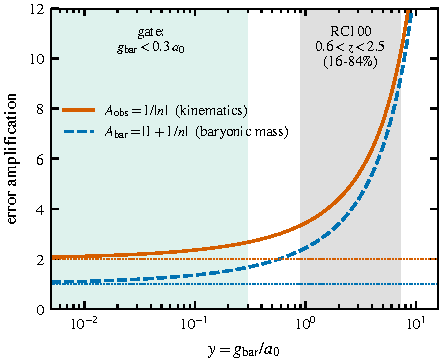
\includegraphics[width=\columnwidth]{fig4_amplification.pdf}
\caption{The factors by which errors in the kinematics ($A_{\rm obs}$, solid) and in the baryonic mass ($A_{\rm bar}$, dashed) are amplified when $a_0$ is inferred through equation~(\ref{eq:invert}). Dotted lines mark the deep limits, 2 and 1. The grey band is the central 68 per cent of the RC100 sample, with the baryonic masses of Section~\ref{sec:existing} (SED stellar mass plus scaling-relation gas); the shaded region on the left is the gate proposed in Section~\ref{sec:design}.}
\label{fig:amp}
\end{figure}

\subsection{What existing data say}
\label{sec:existing}
\emph{RC100 on halo-free baryons.} \citet{NestorShachar2023} tabulate, for 100 galaxies at $0.6<z<2.5$, the circular velocity $V_c$ at the effective radius $R_e$, the stellar mass from fits to the spectral energy distribution (SED), and two outputs of their disc--halo mass models: a fitted baryonic mass and the dark-matter fraction inside $R_e$, $f_{\rm DM}\equiv V_{\rm DM}^2/V_c^2$. We use the published table (table B1 of the journal version). Its redshift, fitted baryonic mass, $R_e$, $f_{\rm DM}$, $V_c$ and velocity dispersion were compared row by row with the journal and with arXiv:2209.12199v1 (one galaxy was refitted between the two). The SED stellar masses that our primary route uses were transcribed from arXiv v1; they equal the journal's column in all 100 rows and agree with the independently tabulated SED masses of \citet{Price2021} to a median of 0.00 dex for the RC41 subsample described below. The fitted baryonic mass and $f_{\rm DM}$ come from a fit that contains a $\Lambda$CDM halo, so our primary route uses neither. We take $M_b=M_*(1+\mu)$, with $M_*$ the tabulated SED stellar mass and $\mu$ the ratio of molecular gas to stars given by the scaling relations of \citet{Tacconi2018} at the galaxy's redshift and stellar mass, place $M_b$ in a thin exponential disc with the tabulated $R_e$, and compute $g_{\rm bar}$ at $R_e$, with $g_{\rm obs}=V_c^2/R_e$. Let $f\equiv1-g_{\rm bar}/g_{\rm obs}$ be the fraction of $g_{\rm obs}$ that the baryons do not supply. By equation~(\ref{eq:nu}), $g_{\rm bar}/g_{\rm obs}=1/\nu=1-e^{-\sqrt y}$. Therefore
\begin{equation}
e^{-\sqrt y}=f\ \Longrightarrow\ y=\Big[\ln\frac1{f}\Big]^2\ \Longrightarrow\ \hat a_0=\frac{(1-f)\,g_{\rm obs}}{[\ln(1/f)]^2} .
\label{eq:rc100}
\end{equation}
In 41 of the 100 galaxies the baryons alone supply all of $g_{\rm obs}$ or more ($g_{\rm bar}\geq g_{\rm obs}$), so no $a_0$ can be inferred: these discs sit at the Newtonian floor, and a censored analysis can carry them only as upper limits, at the value of $\hat a_0$ for $f=0.02$. The floor fraction rises with redshift: 7 of 26 discs (27 per cent) at $0.5<z<1$, 6 of 18 and 7 of 15 at $1<z<2$, and 21 of 41 (51 per cent) at $2<z<2.6$ (a rank correlation of floor membership with $z$ has $p=0.013$). We use the open interval $0.02<f<0.98$, which keeps the other 59 (Fig.~\ref{fig:rc100}a). Their median is $\hat a_0=2.1\times10^{-10}$ m s$^{-2}$, which is biased high because the floor galaxies are excluded, with a scatter of 0.4 dex, as large as Table~\ref{tab:amp} leads one to expect. A straight-line fit to these 59 gives
\begin{equation}
\frac{d\log_{10}\hat a_0}{dz}=-0.12\pm0.10 .
\end{equation}
Laws (b) and (c), fitted in the same way at the same redshifts (the halo law for $10^{12}\,{\rm M_\odot}$, appropriate to these massive discs), have slopes of $+0.23$ and $+0.15$. The inversion itself does not manufacture a flat trend: dark fractions generated from equation~(\ref{eq:nu}) on the real redshifts and accelerations, with injected slopes of 0, $+0.13$ and $+0.23$ and 0.05 of noise in $f$, return those slopes to 0.01. For comparison we also invert the authors' halo-model dark fraction, $f=f_{\rm DM}$, for which $1-f=g_{\rm bar}/g_{\rm obs}$ holds by definition (Fig.~\ref{fig:rc100}b). This comparison route is defined for 99 galaxies and gives a median of $1.5\times10^{-10}$ m s$^{-2}$ and a slope of $-0.09\pm0.06$; the refitted galaxy moves this slope by $0.3\sigma$ and leaves the native route unchanged. The two routes agree within $1\sigma$.

The native slope, however, describes only the discs left in the window, and the window removes discs preferentially at high redshift. Kept as the lowest values, the implied $a_0$ \emph{falls} with redshift (Spearman $\rho=-0.27$, $p=0.006$), and above $z=2$ the median disc is at the floor; a censored (Tobit-type) regression that carries the floor discs as upper limits gives $d\log_{10}\hat a_0/dz=-0.46\pm0.17$, with a scatter of 1.0 dex. No law of Table~\ref{tab:laws} falls. The decision rule of Section~\ref{sec:design} counts a result inconsistent with every law against all of them; the simpler reading is a redshift-dependent bias of the native baryons (SED stellar masses plus scaling-relation gas in a thin disc). On these inputs the route diagnoses the baryon calibration and does not measure $a_0$: its window-only slope is not evidence for constancy. The injection test above, with 0.05 of noise in $f$, models neither baryonic-mass errors of 0.2 dex nor this censoring.

Neither result is a measurement, for five reasons, and we attach no significance to the formal distance between either slope and either comparator. First, the inputs still contain models. The native gas comes from a scaling relation rather than a measurement, and the circular velocities are outputs of the authors' fits, which include a halo. On the comparison route the dark fractions track the authors' baryonic-mass prior: for the RC41 subsample, the galaxies with independently tabulated SED stellar and gas masses \citep{Price2021} (41, of which 16 are among the floor discs above), the residual from a constant $a_0$ correlates with the offset of RC100's fitted baryonic mass from those masses (Spearman $\rho=+0.33$, $p=0.036$). Secondly, RC100's own table is not internally consistent in every row: two galaxies have $V_c^2<3.36\sigma_0^2$ at $R_e$, so that $V_{\rm rot}^2<0$ by their equation 8, and 14 more lie below their cut $V_{\rm rot}/\sigma_0=2.3$ at $R_e$; dropping them moves the comparison slope to $-0.07\pm0.06$, by $0.3\sigma$, and the native slope to $-0.14\pm0.11$. Thirdly, the sample is selected differently at different redshifts: controlling for the measured $g_{\rm obs}$ gives $-0.21\pm0.10$ on the native route and $-0.12\pm0.06$ on the comparison route, and controlling for the inferred $y$ gives $+0.09\pm0.06$ and $+0.02\pm0.05$, a control that also absorbs part of any real signal, since a change of $a_0$ changes $y$.

Fourthly, and decisively, both slopes depend on the redshift calibration of the baryonic masses. Suppose the baryonic masses carry a drift of $\beta$ dex per unit redshift about the mean redshift, so that each $g_{\rm bar}$ is multiplied by $10^{\beta(z-\bar z)}$. A drift of $\beta=-0.05$, a factor of 1.1 at either end of the range, moves the native slope to $+0.02\pm0.09$ and the comparison slope to $+0.04\pm0.06$, both within $1\sigma$ of constancy; on the comparison route the halo law then lies $1.9\sigma$ away ($\beta=-0.075$ brings it within $1\sigma$), and for $\beta=-0.10$ the slope is $+0.17\pm0.07$, within $1\sigma$ of the $H(z)$ law and $2.5\sigma$ from constancy. One galaxy that sits exactly at the edge of the comparison inversion, $f_{\rm DM}=0.02$, moves its slope by $0.4\sigma$ on its own. Fifthly, the pattern is not reproduced by an independent sample. For 117 galaxies of KMOS$^{\rm 3D}$ with circular velocities from \citet{Ubler2017}, sizes from the survey catalogue \citep{Wisnioski2019} and gas masses from scaling relations (93 of them not in RC100), every model leaves residuals that fall with redshift, the constant-$a_0$ model included. The reason is common to all models: at $z>1.9$ between 27 and 54 per cent of these galaxies rotate more slowly than their own Newtonian baryons would require, which no model that adds gravity to the baryons can fit, and on native baryons the same holds for 41 of the 100 RC100 discs. Neither sample therefore decides between the laws of Table~\ref{tab:laws}. Their limiting input is the baryonic mass, and a decisive sample needs gas masses measured galaxy by galaxy.

\emph{The MUSE lensed sample at $z\simeq1$.} Two analyses of one survey point in different directions. \citet{Jeanneau2026} find that the baryonic Tully--Fisher zero point of 95 lensed galaxies at $z\simeq1$ has changed by $0.00\pm0.06$ dex with respect to $z=0$; their atomic and molecular gas masses come from scaling relations and make up a median 70 per cent of $M_b$. \citet{Ciocan2026} fit the radial acceleration relation of 79 galaxies at $0.33<z<1.44$ and find $a_0(z\simeq1)=2.38^{+0.12}_{-0.10}\times10^{-10}$ m s$^{-2}$ (95 per cent interval), a rise faster than the $H(z)$ law: $\Delta\simeq+0.30$ relative to the local $1.2\times10^{-10}$ m s$^{-2}$, and $+0.38$ relative to their own fitted $a_0(0)=1.0\times10^{-10}$ m s$^{-2}$. Taken at face value this is the strongest published result against a constant $a_0$, and we state it as such. It is not, however, independent of how the masses are obtained. The public per-galaxy products of the survey give, for each galaxy, the disc mass fitted jointly with a dark halo, which is the route of \citet{Ciocan2026}, and an independent stellar mass from the spectral energy distribution (SED). Solving equation~(\ref{eq:nu}) for $a_0$ at the effective radius of 109 galaxies in three redshift thirds (Appendix~\ref{app:methods}), the implied $a_0$ rises by $+0.57\pm0.09$ dex between the outer thirds with the fitted masses, against $+0.18$ for the $H(z)$ law. It is not recovered when no quantity from the halo fit enters the baryons, but neither of those routes establishes constancy either. On both, $g_{\rm obs}$ is still the velocity of the DC14 disc--halo model (Appendix~\ref{app:methods}). For a thin disc of the SED stellar mass alone (route iii) the implied $a_0$ changes by $-0.26\pm0.28$ dex. With molecular gas from a scaling relation added (route ii), the implied scale is 0.22 and 0.27 times the local value in the first two thirds, with the baryons exceeding the model's dynamical acceleration in 13 of 37 and 14 of 36 galaxies, and in the highest third they exceed it in 21 of 36, which then admits no $a_0$ at all: against interest, a constant $a_0$ lies outside the 95 per cent interval in two of the three thirds of this route. (Our earlier SED routes, which still normalised the baryons with the fit's dark fraction and disc mass, gave $-0.11\pm0.49$ and $+0.04\pm0.14$ dex.) The data cannot say which masses are biased: the fitted minus SED stellar mass falls by 0.72 dex per unit redshift (95 per cent interval 0.50--0.97), and by 0.43 dex (0.15--0.72) at fixed SED stellar mass; on those earlier SED routes, restoring the rise would have needed an SED-mass bias of 1.8--2.2 dex per unit redshift. The rise is route-dependent: neither it nor constancy is established. At $z\simeq1$ the halo-emergent law cannot in any case be told from constancy (Table~\ref{tab:laws}).

\emph{Outer rotation curves at $z\simeq1.5$.} KURVS-CDFS \citep{Puglisi2023} follows star-forming discs to about four effective radii. For the ten discs with tabulated dark-matter fractions the outermost points lie at $g_{\rm bar}/a_0=0.06$--$0.67$ for the survey's own gas fractions, the first public sample in the regime the test needs. At those radii the observed velocities must be corrected for pressure support, and the result turns on that correction and on the unmeasured gas. With the correction calibrated on simulations by \citet{Kretschmer2021} and the survey's molecular-gas estimate, at a grid cell declared before this comparison (although after an earlier pressure model had been scored, so the choice of calibration was not blind; Appendix~\ref{app:methods}), the outer accelerations exceed the constant-$a_0$ prediction by $3.3\sigma$, while the rival's central value sits at zero ($-0.1\sigma$). We report this against interest. It is not a detection. The outer velocities tabulated by the survey are its model curve evaluated at the last radius; with the measured outermost points the two numbers become $+2.4\sigma$ and $-0.4\sigma$. The lean disappears for a common velocity scale 4.5 per cent lower and for a pressure correction at 0.6 of the calibration ($+1.3\sigma$ and $-2.0\sigma$), and it reverses for a cold-gas mass of 1.5 times the stellar mass ($+1.2\sigma$ and $-2.1\sigma$). With gas and pressure support treated as nuisance parameters the likelihood ratio between the two laws is 0.5--1.7. The lean also needs the calibration of \citet{Kretschmer2021}, which comes from $\Lambda$CDM simulations. With the measured points and, in its place, the analytic correction for an exponential disc, $\alpha=2R/R_d$ with the measured dispersion, both laws under-predict the outer accelerations, constancy by $+0.38\pm0.06$ dex ($6.8\sigma$) and the rival by $+0.23\pm0.05$ dex ($4.3\sigma$), so the rival is the closer; over six sets of outer points and four analytic prescriptions (from no correction to one using the measured dispersion gradient), 4 cells lean towards constancy, 7 towards the rival and 13 towards neither. Without the simulation calibration, then, the lean towards the rival weakens but more cells still point that way than towards constancy. What would settle it is the discs' own cold gas and their outer pressure support, both measurable.

\emph{H\,{\sc i} rotation curves at $z<0.1$.} \citet{Varasteanu2026} fit the radial acceleration relation of 130 resolved H\,{\sc i}-selected galaxies out to $z\approx0.09$. Over that range $a_0\propto H(z)$ changes $a_0$ by only 4.5 per cent, so the sample cannot separate the laws: its own linear trend, $a_1/a_0=-1.04\pm1.51$ per unit redshift, is consistent with constancy ($-0.7\sigma$) and with $H(z)$ ($-1.0\sigma$). Anchored to SPARC at $z=0$ the fitted trend becomes a formal $5\sigma$ rise; in their own table it is $(+5.23\pm1.05)\times10^{-10}$ m s$^{-2}$ per unit redshift with mass-to-light ratios that vary between galaxies and $(-4.80\pm0.76)\times10^{-10}$ with a constant ratio of 0.6. The authors find no significant evolution of the acceleration scale within their sample and attribute an apparent trend of the Tully--Fisher zero point ($8.7\sigma$ in the forward fit, $3.4\sigma$ in their fiducial inverse fit) to selection; the earlier 19-galaxy analysis reported tentative evidence for evolution \citep{Varasteanu2025}. In post hoc runs of a declared MIGHTEE-like scenario in our repository (SPARC-resampled mock samples, not the survey's data; Appendix~\ref{app:methods}), the formal error of the anchored trend was 5.2 times smaller than its scatter, and a constant $a_0$ gave a formal $z>3$ in 11 to 32 per cent of the mocks. None of this is evidence for constancy or against it.

\emph{Discs at $z\simeq2.5$--14.} Every further public sample at these redshifts that we could assemble has been scored under criteria fixed before the scoring \citep{Zimmerman2026wall}, and none measures $a_0$. The discs with measured gas are massive and their last measured radii lie close to the Newtonian regime, where Table~\ref{tab:amp} multiplies every baryonic-mass error several-fold; the discs that reach low accelerations have no gas measurement; and in several the published baryons alone exceed the dynamics. Pools of the published objects at $z\geq4$ with both stellar and gas masses do not separate the two laws once the common baryonic-mass calibration is uncertain by 0.30 dex, and pools with stellar masses only, which appear to separate them, lie above both predictions, in the direction the missing gas would remove. The repository analysis behind this paragraph fails one of its own frozen controls (a recomputation of committed residuals agrees only to $2\times10^{-3}$ dex against a $10^{-4}$ tolerance), so we cite it only qualitatively.

\emph{Native inputs at $z\simeq2$--5.} Two points that appeared to exclude a constant $a_0$ in an earlier compilation of implied $a_0$ against redshift in our repository (Appendix~\ref{app:repro}), whose CRISTAL point took its baryons from the authors' disc--halo fits, do not survive baryonic masses free of halo fits (SED stellar masses plus measured or scaling-relation gas, in a declared thin disc; Appendix~\ref{app:methods}). For the CRISTAL discs at $4<z<6$ \citep{Lee2025}, no point excludes a constant $a_0$ at 95 per cent, and over 1008 declared variants of gas, stellar mass, pressure support, inclination, radius and sample, $a_0\propto H(z)$ is excluded in 59 per cent of cells and constancy in 24 per cent, which does not discriminate. The one massive disc at $z\simeq2$ in our census whose implied $a_0$ lay above the constant value is ALESS 122.1 at $z=2.02$, with kinematics from \citet{Amvrosiadis2025}, the velocity dispersion of \citet{CalistroRivera2018} and the multi-tracer gas calibration of \citet{Dunne2022}. Its primary native scale is 8.8 times the local value, but across the declared choices of gas tracer, radius and pressure term it ranges from no solution to about 20 times that value: over 540 variants no inferred value survives in 44 per cent, constancy is excluded in 27 per cent (always from above) and $a_0\propto H(z)$ in 15 per cent, which, as for CRISTAL, does not discriminate.

\emph{Rotation curves at $z\sim2$.} \citet{Milgrom2017} showed that the outer rotation curves of the massive discs of \citet{Genzel2017} are compatible with the local $a_0$ and all but exclude a value about four times larger. Law (b) predicts a factor of 3.0 at $z=2$; whether those data disfavour it would need the calibration analysis applied to RC100 above, and they are subject to the same limits: high accelerations and model-dependent baryonic masses.

\emph{Summary.} The existing rotation curves at $z\simeq1$--14 decide nothing between the laws of Table~\ref{tab:laws}. In every case the limiting input is the baryonic mass, and above all its common calibration. At $z\gtrsim2$ the gas masses come from scaling relations \citep{Tacconi2018,Tacconi2020} or from CO with a conversion factor whose metallicity dependence is uncertain \citep{Bolatto2013}. The dust-to-molecular-gas ratios of the ACE survey at $z\simeq2.2$ \citep{Geesink2026}, each source with its own conversions, lie 0.2--0.7 dex below the local relation of \citet{Bertemes2018} at the same metallicity, depending on how that relation is extrapolated in metallicity (Appendix~\ref{app:methods}; \citealt{Zimmerman2026wall}). No calibration independent of the dynamics under test is known to reach 0.1 dex.

\begin{figure}
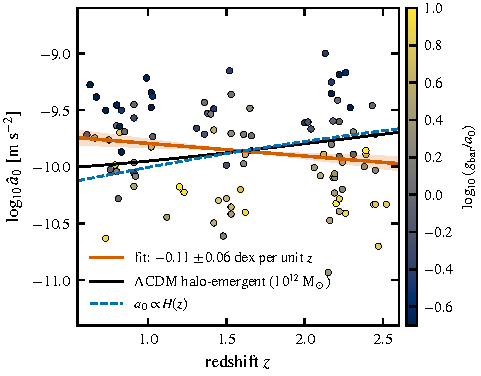
\includegraphics[width=\columnwidth]{fig5_rc100.pdf}
\caption{The acceleration scale inferred for RC100 (published table) through equation~(\ref{eq:rc100}), coloured by the acceleration at which each galaxy is measured. (a) The halo-free route: baryonic masses from the SED stellar masses plus scaling-relation gas, for the 59 galaxies whose baryons do not already supply the observed acceleration. The 41 at the Newtonian floor cannot be inverted and are not shown; their share rises from 27 per cent at $z<1$ to 51 per cent at $z>2$, so this panel is a censored sample and its trend is not a measurement of $a_0$ (Section~\ref{sec:existing}). (b) The comparison route, which uses the authors' halo-model dark fraction $f_{\rm DM}$, for 99 galaxies. Bands are the fitted trends with their $1\sigma$ slope errors. The thin solid and dashed lines are the halo-emergent ($10^{12}\,{\rm M_\odot}$) and $H(z)$ laws, normalised at the mean redshift. The anticorrelation of $\hat a_0$ with $y$ is the signature of noise in $f$, which moves the two in opposite directions. Both trends are conditional on the redshift calibration of the baryonic masses (Section~\ref{sec:existing}): a drift of $-0.05$ dex per unit redshift moves them to $+0.02\pm0.09$ and $+0.04\pm0.06$.}
\label{fig:rc100}
\end{figure}

\subsection{The measurement that decides}
\label{sec:design}
\emph{The gate.} Table~\ref{tab:amp} shows that a galaxy is useful only if it is measured at low acceleration. We propose $g_{\rm bar}(R_{\rm out})<0.3a_0$, where $A_{\rm obs}\le2.7$ and $A_{\rm bar}\le1.7$. With $g_{\rm bar}=\Gamma GM_b/R^2$, $\Gamma\simeq1.2$ and $a_0$ the working value of equation~(\ref{eq:a0value}), this reads
\begin{equation}
M_b<1.7\times10^{8}\,{\rm M_\odot}\,\Big(\frac{R_{\rm out}}{\rm kpc}\Big)^2 ,
\end{equation}
for example $M_b=5\times10^{9}\,{\rm M_\odot}$ traced to 6 kpc. Such galaxies rotate at $V_f\simeq83$--$125$ km s$^{-1}$, which fixes the halo mass and so the decision value of equation~(\ref{eq:dgate}). At $z\simeq2.5$ they can be resolved only with the help of gravitational lensing, which adds a requirement on the lens model: a magnification uncertainty below about 0.05 dex (see the budget below). Rotation must dominate ($V/\sigma>1.5$ from a forward-modelled fit), the inclination should be between $35^\circ$ and $75^\circ$, and the gas mass must be measured and not inferred from a scaling relation. A practical sequence is a JWST NIRSpec integral-field observation first, to establish rotation and bound the acceleration (H$\alpha$ and [O\,{\sc iii}] fall together in the G235H grating for $2.3<z<3.8$), followed by ALMA CO(3--2), which falls in Band 3 for $2.0<z<3.1$ and gives the molecular gas mass and a second kinematic tracer. We know of no published object that passes every gate. In a ledger of candidates re-derived from the primary papers, the only object at $z\geq2$ that could pass the acceleration gate is OLAS M0717-02064 \citep{Hirtenstein2019}: $z=2.07$, magnification 6.5, $\log_{10}M_*/{\rm M_\odot}=8.1$, and rotation-supported with $v/\sigma=1.6$. It lies just below the preferred redshift window, where Table~\ref{tab:laws} still separates the laws by 0.16 dex for the gate's haloes, and it has not been observed with JWST. Its gas mass and the uncertainty of its lens model are not yet measured.

\emph{How many galaxies?} Each galaxy that passes the gate gives $\Delta_i=\log_{10}[\hat a_0/a_0(0)]$. Under constancy $\Delta_i$ is drawn from a normal distribution of mean 0 and variance $s_0^2=\sigma_{\rm m}^2+\sigma_{\rm int}^2$, where $\sigma_{\rm m}$ is the measurement error and $\sigma_{\rm int}$ is the intrinsic scatter of the relation, about 0.034 dex in $g_{\rm obs}$ \citep{Desmond2023}, which equation~(\ref{eq:amp}) amplifies to 0.09 dex in $\hat a_0$ at $y=0.3$. Under the halo law the mean is $\Delta=+0.22$ and the variance $s_1^2=s_0^2+\sigma_{\rm h}^2$, where $\sigma_{\rm h}=0.13$ dex is the halo-to-halo scatter of 0.11 dex in concentration \citep{DuttonMaccio2014} propagated through equation~(\ref{eq:lawhalo}) at the gate's halo mass. For two exactly specified predictions with one Gaussian error $\sigma$, the expected logarithm of the likelihood ratio is $\Delta^2/2\sigma^2$, so expected odds of 20:1 \citep[strong evidence on the scale of][]{KassRaftery1995} need $\sigma\le\Delta/\sqrt{2\ln20}=\Delta/2.45$, that is 0.088 dex for the halo law and 0.24 dex for $H(z)$. With both scatters the expected log-odds from $N$ galaxies when constancy is true are
\begin{equation}
\langle\ln B\rangle=N\Big[\ln\frac{s_1}{s_0}-\frac12+\frac{s_0^2+\Delta^2}{2s_1^2}\Big],
\label{eq:lnB}
\end{equation}
and the expression with $s_0\leftrightarrow s_1$ applies when the halo law is true. We call $\exp\langle\ln B\rangle$, the smaller of the two, the expected odds. Expected odds are not the probability of reaching them: at the idealised limit of equation~(\ref{eq:lnB}) with one pair of point hypotheses, $\ln B$ is normally distributed about $\ln20$ and reaches 20:1 only half the time, pointing the wrong way 11 per cent of the time. We therefore also give, from a Monte Carlo of the exact likelihood ratio, the probability of reaching 20:1 under each hypothesis and of evidence pointing the wrong way ($\ln B<0$). Table~\ref{tab:odds} gives the design. One galaxy at 0.13 dex yields 1.8:1. Expected odds of 20:1 need five galaxies at 0.10 or 0.13 dex, or eight at 0.20 dex, and at those $N$ the chance of actually reaching 20:1 is only 0.53--0.68 under the less favourable hypothesis, with misleading evidence in up to 10 per cent of trials; reaching 20:1 with 90 per cent probability needs 9, 12 and 20 galaxies. The designs of an earlier deposited version of this test \citep{Zimmerman2026a0z} and of the previous draft of this paper, which used the rise of a $10^{12}\,{\rm M_\odot}$ halo, are superseded: at the gate's halo mass, two galaxies at 0.10 dex give 4.4:1 and four at 0.20 dex give 4.5:1.

The $\Lambda$CDM prediction is itself uncertain. We carry the choice of concentration--mass relation as a composite hypothesis: under the halo law, $\Delta$ itself is drawn once for the whole sample from a normal distribution centred on $+0.22$ with width $\sigma_{\rm sys}$, a term that does not average down. The relations of \citet{DuttonMaccio2014} and \citet{Duffy2008} differ by 0.22 dex at the gate's halo mass. With $\sigma_{\rm sys}=0.10$ dex, which allows the rise to be lower as well as higher, eight galaxies at 0.20 dex become 27; with $0.20$ dex, 48 (Table~\ref{tab:odds}). The relation spread, not the measurement error, is then the limiting term.

\begin{table*}
\caption{The design at the gated decision value ($\Delta=+0.22$ dex at $z=2.5$), for $N$ galaxies passing the gate, each with measurement error $\sigma_{\rm m}$ on $\log_{10}\hat a_0$, with intrinsic (0.09 dex) and halo-to-halo (0.13 dex) scatter and independent mass errors. $N_{20}$: the smallest $N$ with expected odds $\exp\langle\ln B\rangle\geq20$, the smaller of the two cases (constancy true; halo law true). $P_{20}$: the probability of reaching 20:1 at $N_{20}$ under the less favourable hypothesis. $P_{\rm wrong}$: the probability that the evidence points the wrong way at $N_{20}$, under the more exposed hypothesis. $N_{90}$: the smallest $N$ that reaches 20:1 with probability 0.9 under both hypotheses. Columns 6--9: the same with the $\Lambda$CDM prediction uncertain by a width $\sigma_{\rm sys}$ shared by the sample (Section~\ref{sec:design}). Probabilities from $2\times10^4$--$10^5$ Monte Carlo samples.}
\label{tab:odds}
\begin{tabular}{ccccccccc}
\toprule
 & \multicolumn{4}{c}{$\sigma_{\rm sys}=0$} & \multicolumn{2}{c}{$\sigma_{\rm sys}=0.10$ dex} & \multicolumn{2}{c}{$\sigma_{\rm sys}=0.20$ dex}\\
$\sigma_{\rm m}$ [dex] & $N_{20}$ & $P_{20}$ & $P_{\rm wrong}$ & $N_{90}$ & $N_{20}$ & $N_{90}$ & $N_{20}$ & $N_{90}$\\
\midrule
0.10 & 5 & 0.68 & 0.07 & 9 & 10 & 29 & 14 & 40\\
0.13 & 5 & 0.55 & 0.10 & 12 & 13 & 44 & 20 & 63\\
0.20 & 8 & 0.53 & 0.10 & 20 & 27 & 110 & 48 & 167\\
\bottomrule
\end{tabular}
\end{table*}

\emph{The error budget.} Gravitational lensing conserves surface brightness, so $g_{\rm bar}\propto M_b/R^2$ does not depend on the magnification $\mu$, while $g_{\rm obs}=V^2/R$ scales as $\mu^{1/2}$ through the radius. Equation~(\ref{eq:amp}) then gives
\begin{equation}
\sigma_{\rm m}^2=A_{\rm obs}^2\Big[\Big(\frac{2}{\ln10}\frac{\delta V}{V}\Big)^2+\Big(\frac12\delta\log_{10}\mu\Big)^2\Big]+A_{\rm bar}^2\big(\delta\log_{10}M_b\big)^2 ,
\end{equation}
where $\delta\log_{10}M_b$ is the error of the mass scale at fixed magnification. At $y=0.2$ ($A_{\rm obs}=2.5$, $A_{\rm bar}=1.5$), three budgets reproduce the rows of Table~\ref{tab:odds}: $\sigma_{\rm m}=0.10$ dex needs $(\delta V/V,\delta\log_{10}M_b,\delta\log_{10}\mu)=(2.5$ per cent$,0.04,0.04)$; $0.13$ dex needs $(3$ per cent$,0.06,0.05)$; and $0.20$ dex needs $(5$ per cent$,0.10,0.06)$. The first two are beyond present practice for the baryonic mass, since the conversion from CO luminosity to molecular mass is rarely known to 0.06 dex. The third is within reach. The realistic programme is therefore about eight galaxies at 0.20 dex for expected odds of 20:1, and about twenty for a 90 per cent chance of reaching them, provided that their mass errors are independent, which the next paragraph examines.

\emph{A common calibration does not average down.} Part of $\delta\log_{10}M_b$ is shared by the whole sample: the conversion from CO luminosity to molecular mass, the dust-to-gas ratio and the zero point of the stellar masses. A shared error $\delta_c$ on $\log_{10}M_b$ adds the same $\sigma_C=A_{\rm bar}\delta_c$ to every galaxy. The covariance of the $N$ values of $\Delta_i$ is then $s^2\mathbf{I}+\sigma_C^2\mathbf{J}$, with $\mathbf{J}$ the matrix of ones and $s^2$ the per-galaxy variance of equation~(\ref{eq:lnB}), and the expected log-odds are the Kullback--Leibler divergence between two $N$-dimensional normal distributions, which reduces to equation~(\ref{eq:lnB}) when $\sigma_C=0$. Along the direction of the mean the variance is $s^2/N+\sigma_C^2$, so the separation of the sample means cannot exceed $\Delta/\sigma_C$ however many galaxies are observed. Table~\ref{tab:shared} gives the result at $y=0.2$, where $A_{\rm bar}=1.52$. A common error of 0.10 dex reduces eight galaxies at 0.20 dex from 20:1 to 2.5:1 against the halo law. Odds of 20:1 from the sample means require $\delta_c\le0.06$ dex against the halo law and $\delta_c\le0.15$ dex against the $H(z)$ law. Those limits are reached only as $N\to\infty$, so the eight-galaxy design and the 0.06 dex limit are not jointly sufficient: on the same computation, eight galaxies at 0.20 dex give 8.3:1 at $\delta_c=0.04$ dex and 4.8:1 at 0.06 dex, and expected odds of 20:1 against the halo law need 14, 20 and 34 galaxies at $\delta_c=0.04$, 0.05 and 0.06 dex (64 at 0.05 dex if the concentration--mass relation is also carried with $\sigma_{\rm sys}=0.10$ dex). The gas-calibration spread of Section~\ref{sec:existing}, 0.2--0.7 dex at $z\approx2.2$, is 0.09--0.48 dex in $M_b$ for a gas fraction of one half. The deciding measurement therefore needs, besides the galaxies, a calibration of the gas mass at $z\approx2.5$ that does not exist today.

\begin{table}
\caption{Expected odds with a baryonic-mass calibration error $\delta_c$ shared by every galaxy, at $y=0.2$ ($\sigma_C=A_{\rm bar}\delta_c$, $A_{\rm bar}=1.52$), with the intrinsic and halo-to-halo scatter of Table~\ref{tab:odds}. Columns 3--6: eight galaxies at $\sigma_{\rm m}=0.20$ dex (with $P_{20}$, the probability of reaching 20:1 under the less favourable hypothesis) and five at 0.10 dex against the gated halo law ($\Delta=0.22$), and eight at 0.20 dex against the $H(z)$ law ($\Delta=0.58$). Columns 7--8: $\Delta/\sigma_C$, the largest separation of the sample means in standard deviations for any number of galaxies.}
\label{tab:shared}
\setlength{\tabcolsep}{2.8pt}
\begin{tabular}{@{}cccccccc@{}}
\toprule
$\delta_c$ & $\sigma_C$ & \multicolumn{2}{c}{halo, 8@0.20} & halo, 5@0.10 & $H(z)$, 8@0.20 & halo & $H(z)$\\
{[dex]} & {[dex]} & odds & $P_{20}$ & odds & odds & \multicolumn{2}{c}{$\Delta/\sigma_C$}\\
\midrule
0.00 & 0.000 & 20:1 & 0.53 & 40:1 & $9.1\times10^{11}$:1 & -- & --\\
0.05 & 0.076 & 6.2:1 & 0.26 & 9.0:1 & $1.3\times10^{6}$:1 & 2.8 & 7.6\\
0.10 & 0.152 & 2.5:1 & 0.04 & 3.2:1 & 290:1 & 1.4 & 3.8\\
0.15 & 0.228 & 1.7:1 & 0.00 & 2.2:1 & 17:1 & 0.9 & 2.5\\
0.20 & 0.304 & 1.5:1 & 0.00 & 1.9:1 & 5.4:1 & 0.7 & 1.9\\
\bottomrule
\end{tabular}
\end{table}

\emph{Why the calibration must come from outside.} In the deep limit $g_{\rm obs}$ depends on a common mass-calibration factor $f$ and on $a_0$ only through their product $fa_0$, so a sample of deep galaxies measures little more than $fa_0$. The two can be separated by the rotation curves alone only through the curvature of equation~(\ref{eq:nu}), which needs points on both sides of the bend. With $f$ free, the Fisher matrix gives $\sigma(\log_{10}a_0)\geq3\sigma/\sqrt N$ for any design with $N$ points of error $\sigma$; for 20 points at 0.1 dex spread evenly in $\log y$, the estimate stays below 0.1 dex only if they run from $y=0.001$ to at least $y\simeq17$, reaches 0.096 dex at best if they start at $y=0.01$, and never reaches 0.1 dex if they start at $y=0.1$. These statements are formalised, as implications of the assumed law, in a companion note \citep{Zimmerman2026wall}; we have recomputed the numbers for equation~(\ref{eq:nu}). There are thus two routes: rotation curves that span the bend widely enough to calibrate $f$ themselves, which no curve at high redshift does (it would need about four decades in $y$), or an external calibration of $f$ to better than 0.1 dex. The gate of this section selects deep galaxies and so takes the second route. This reconciles the design above, whose odds assume independent mass errors, with that note's conclusion that in every existing test the limit that survives an unlimited sample is the calibration of the baryonic masses: the two agree once the shared part of the calibration is carried, as in Table~\ref{tab:shared}.

\emph{The decision rule.} The statistic is the mean of $\Delta_i$ over the galaxies that pass the gate, with $\hat a_0$ from equation~(\ref{eq:invert}) and $a_0(0)$ fixed beforehand from the local relation using the same mass-to-light conventions. A result near $0$ supports constancy: law (a), and with it plain MOND. A result near $+0.22$ or above supports an emergent or $H(z)$-coupled scale and excludes equation~(\ref{eq:relation}) with a constant $\rho_\Lambda$. A result inconsistent with all of them counts against all of them. No nuisance term may be introduced after the data are seen. Because $a_0(0)$ and $\hat a_0(z)$ are obtained with the same function and conventions, the test does not depend on $\kappa$ or on $H_0$, and it depends on the choice of transition function only weakly provided $a_0(0)$ is calibrated on local galaxies at matching accelerations. It does depend on the stellar and gas mass scales being on a common calibration at both epochs (Table~\ref{tab:shared}).

%=====================================================================================================================
\section{What the relation does not explain}
\label{sec:limits}
\emph{The coefficient is not derived.} We know of no derivation of $\kappa=1/2$. The simplest physical identification, equating the Unruh temperature of $a_0$ with the temperature of the de Sitter horizon, gives $a_0=cH_\Lambda$, which is six times too large; the form $cH_\Lambda/2\pi$ ($\kappa=0.461$) is allowed by the data as readily as $1/2$ (Table~\ref{tab:cands}), and on a common $H_0$ footing Milgrom's $cH_0/2\pi$ fits SPARC at least as well as $\tfrac12c\sqrt{G\rho_{\rm crit}}$ (Section~\ref{sec:measure}); $\kappa=1/2$ is a fitted value. \ifpapersix A separate analysis finds that, in the aether--scalar class of local relativistic actions it examined, the additive constant of the MOND Lagrangian is degenerate with $\Lambda$, so those actions do not fix the coefficient \citep[its four-form section is superseded]{Zimmerman2026kappa}. \fi Nothing in the redshift test changes if $\kappa$ lies anywhere in 0.4--0.6.

\emph{A scale is not a dynamics.} Equation~(\ref{eq:relation}) fixes a number. It does not say whether the low-acceleration behaviour of galaxies is a modification of gravity, a modification of inertia, or a regularity of dark matter. It is therefore silent on gravitational lensing, the cosmic microwave background, the growth of structure, the external field effect \citep{Chae2020} and the Solar System. Nor does it remove the need for the cold matter whose density the microwave background and the growth of structure measure: that mass is still required. In particular, equation~(\ref{eq:nu}) is used here only to describe rotation curves; read as a modified-gravity law and extrapolated to Solar System accelerations it is constrained by planetary ephemerides \citep{Hees2016}.

\emph{Clusters of galaxies.} Dynamics governed by $a_0$ leave a residual mass discrepancy of about a factor of two in rich clusters \citep{SandersMcGaugh2002,FamaeyMcGaugh2012}. Anchoring $a_0$ to $\Lambda$ does not change that.

\emph{The mass-to-light ratio.} The value $\kappa=1/2$ with $\rho_\Lambda$ is tenable only if $\Upsilon_{\rm disc}\simeq0.56$ at 3.6 $\mu$m on the Planck-consistent distances (0.62 on the tabulated distances; Table~\ref{tab:upsilon}). An independent determination well outside $0.45$--$0.75$ would exclude it. The $\rho_{\rm crit}$ reading needs $\Upsilon_{\rm disc}\simeq0.47$ (0.52). The deep regime shows how much is at stake: with the SED ratios of MIGHTEE-HI, a $K_s$-band median of 0.35, the coefficient is $0.90\pm0.07$, and with a fixed $\Upsilon_K=0.6$ it is $0.58\pm0.05$ (Section~\ref{sec:deepregime}). The stellar mass calibration, not the number of galaxies, limits this test.

\emph{Constancy is shared.} A constant $a_0$ at $z=2.5$ would not distinguish equation~(\ref{eq:relation}) from a MOND constant of unknown origin. It would exclude the coupling to $H(z)$, which the coincidence $a_0\sim cH_0$ has suggested since 1983, and it would be in tension with the halo-based expectation of Section~\ref{sec:laws}, although the scale inferred for galaxies at fixed baryonic mass need not follow the central acceleration of a fixed-mass halo, so a constant result would constrain $\Lambda$CDM only through such a calibration.

\emph{Dark energy may not be a constant.} If the evidence for evolving dark energy \citep{DESI2025} is confirmed, $\rho_\Lambda$ in equation~(\ref{eq:relation}) will need redefinition. The redshift test is insensitive to this at the level of 0.1 dex (Section~\ref{sec:laws}d).

%=====================================================================================================================
\section{Conclusions}
\label{sec:conc}
\begin{enumerate}
\item The only acceleration that can be formed from $c$, $G$ and the density of the cosmological constant is $\kappa c\sqrt{G\rho_\Lambda}$. For $\kappa=1/2$ it is $9.36\times10^{-11}$ m s$^{-2}$; the same expression with the critical density is $1.13\times10^{-10}$ m s$^{-2}$. Its equivalent forms are identities and carry no separate evidence.
\item On SPARC, with the Hubble-flow distances on the $H_0$ used for $\rho_\Lambda$, three estimators give $\kappa=0.450\pm0.073$ (Tully--Fisher intercept with its finite-depth correction), $0.58\pm0.18$ (shape only, immune to a common distance error but fragile to the bulge mass-to-light ratio) and $0.43\pm0.08$ (profile likelihood with the mass-to-light ratio free per galaxy). The value $1/2$ is consistent with all three, as are $cH_\Lambda/2\pi$ and $cH_0/2\pi$; on either common footing Milgrom's $2\pi$ form is at least as close to the data as $1/2$. Against that, the joint inference of \citet{Desmond2023} puts $1/2$ at $2.6\sigma$ on the $\rho_\Lambda$ footing. Each estimator's value depends on the $H_0$ convention by up to 0.1, and injection tests show that each returns a known $a_0$. The thermal identifications $cH_\Lambda$ and $2cH_\Lambda$ are excluded.
\item In the deep regime, $g_{\rm bar}<0.2a_0$, the per-galaxy slope of SPARC and MIGHTEE-HI agrees with the slope of equation~(\ref{eq:nu}) at the sampled accelerations, within 0.1--$1.6\sigma$, and excludes a slope of 0.75 at more than $4\sigma$. The amplitude follows the stellar mass-to-light convention: $\kappa_\Lambda=0.90\pm0.07$ with the SED ratios of MIGHTEE-HI and $0.58\pm0.05$ with its fixed $\Upsilon_K=0.6$. Mass-to-light ratios fitted to the rotation curves without the relation lower the deep-regime value by a factor of 1.7 to 2.2 and must not be used.
\item Because stellar and gas masses sum to the baryonic mass, the two calibrations trade against each other and leave a floor $s_\Upsilon s_g/(s_\Upsilon^2+s_g^2)^{1/2}=9.5$ per cent on $a_0$ that no sample size removes. Separating $1/2$ from $0.461$ needs 2.6 per cent. At fixed $\Omega_\Lambda$ only the product $\kappa H_0$ enters the prediction, so $\kappa$ cannot be quoted without $H_0$.
\item The $\Lambda$ anchor predicts a constant $a_0$. A critical-density anchor predicts $+0.58$ dex at $z=2.5$. $\Lambda$CDM haloes predict a rise that depends on halo mass; for the haloes of discs that can be measured at low acceleration it is $+0.22$ dex, with a model systematic of about 0.2 dex from the concentration--mass relation. Inferring $a_0$ from one galaxy amplifies kinematic errors by $1/|n|$ and mass errors by $1/|n|-1$, factors of 5 and 4 at the accelerations of existing high-redshift samples, which is why those samples do not decide the matter.
\item On baryonic masses free of halo fits (SED stellar masses plus scaling-relation gas), the baryons of 41 of the 100 RC100 discs exceed the dynamics, a fraction that rises from 27 per cent at $z<1$ to 51 per cent at $z>2$. The 59 that can be inverted give $d\log_{10}a_0/dz=-0.12\pm0.10$, but with the floor discs kept the implied $a_0$ falls with redshift, which no law predicts: on these inputs the route measures the baryon calibration, not $a_0$, and its lack of a rise is not support for constancy. Inverting the authors' halo-model dark fractions instead gives $-0.09\pm0.06$; a drift of $-0.05$ dex per unit redshift in the baryonic-mass calibration erases either trend, and an independent KMOS$^{\rm 3D}$ sample does not reproduce the pattern. The MUSE-DARK rise of $a_0$ at $z\simeq1$, the strongest published result against constancy, is not recovered with SED stellar masses; with molecular gas added the baryons exceed the model dynamics and constancy lies outside the 95 per cent interval in two of three redshift thirds. The data cannot say which masses are biased. The lean towards $a_0\propto H(z)$ in KURVS at $z\simeq1.5$ rests on a simulation-calibrated pressure correction, the gas and the velocity scale; with analytic corrections both laws under-predict the outer accelerations, the rival by less. On the same native inputs no CRISTAL point at $z\simeq5$ excludes constancy, and neither CRISTAL nor ALESS 122.1 separates the laws. MIGHTEE-HI/LADUMA cannot separate them either, and no sample at $z\simeq2.5$--14 measures $a_0$.
\item About eight lensed rotators at $z\simeq2.5$ with $g_{\rm bar}<0.3a_0$, each measured to 0.20 dex in $a_0$ (five at 0.10 dex), give expected odds of 20:1 between constancy and the halo-emergent rise once intrinsic and halo-to-halo scatter are included, provided their baryonic masses share no calibration error; reaching 20:1 with 90 per cent probability needs about twenty (nine), and carrying the concentration--mass relation as a shared systematic of 0.1 dex raises these numbers by factors of two to five. A baryonic-mass calibration shared by the sample does not average down: at 0.05 and 0.06 dex it raises the eight to 20 and 34, and beyond 0.06 dex (0.15 dex against the $H(z)$ law) the sample means alone cannot reach 20:1 however many galaxies are observed. That calibration cannot come from the rotation curves themselves; the gas prescriptions in use at $z\approx2.2$ differ by 0.2--0.7 dex. A calibrated gas mass is the input still missing.
\end{enumerate}

\section*{Acknowledgements}
% AI disclosure finalised 2026-10-02 from the author's statement of the models used (SUBMISSION_CHECKLIST.md, section 0).
Generative artificial-intelligence tools were used in this work. Large language models from several providers assisted with the derivations, with transcribing and digitising published tables and figures, with writing the analysis code and with drafting the text: Anthropic's Claude (used mainly through the Claude Code tool), models from OpenAI, DeepSeek, Zhipu AI's GLM, Alibaba's Qwen and Google's Gemini. Among the inputs, the digitised MIGHTEE-HI points and the rotation-curve compilation behind the pitfall row of Section~\ref{sec:deepregime} were first produced with DeepSeek and GLM models respectively; both were checked against their sources by script. Every quantitative statement is produced by a public script whose checks can fail, and the author has reviewed the full content and takes sole responsibility for it. The ordering of the observing sequence in Section~\ref{sec:design} was first suggested in an exchange with an OpenAI model. This work made use of the SPARC database \citep{Lelli2016}, of the tables of \citet{NestorShachar2023}, \citet{Price2021}, \citet{Puglisi2023} and \citet{Lee2025}, of the ALESS 122.1 measurements of \citet{Amvrosiadis2025}, \citet{CalistroRivera2018} and \citet{Dunne2022}, of the public per-galaxy products of the MUSE-DARK survey \citep{Ciocan2026}, and of the published fits of \citet{Varasteanu2026}. The author received no funding for this work and declares no conflict of interest.

\section*{Data Availability}
All scripts and outputs are in the public repository \url{https://github.com/carlzimmerman/zimmerman-formula}, in the directory \nolinkurl{qwen_claude_field_theory/papers_2026/mnras_submission_2026_v3} (Appendix~\ref{app:repro}); the version used for this paper is the tagged release \texttt{mnras-v3.3}. The SPARC data are available at \url{http://astroweb.cwru.edu/SPARC/}. The RC100 table is from \citet{NestorShachar2023}; we use the published table (table B1 of the journal version; \nolinkurl{real_research/data/rc100_nestorshachar2023_table3_PUBLISHED.csv}). Its redshift, fitted baryonic mass, $R_e$, $f_{\rm DM}$, $V_c$ and $\sigma_0$ columns were compared row by row with the journal and with table 3 of arXiv:2209.12199v1; the SED stellar masses (column 6), transcribed from arXiv v1, were compared with the journal's column separately (\nolinkurl{real_research/data/rc100_nestorshachar2023_tableB1_logMstar_JOURNAL.csv}) and agree in all 100 rows; the other columns were not compared. The two versions differ in one galaxy, J0901+1814, which was refitted between them, and our earlier transcription of the arXiv table also had one mistyped velocity dispersion; the refit moves the comparison slope of Section~\ref{sec:existing} by $0.3\sigma$ towards zero and does not change the native route. A still earlier transcription had 17 wrong cells, corrected before the previous version of this paper. The MIGHTEE-HI points were digitised from \citet{Varasteanu2025}, and the digitised values are in the repository. The published tables behind the high-redshift analyses (22 sources, including RC100, the KMOS$^{\rm 3D}$ release, MUSE-DARK and MIGHTEE-HI/LADUMA, but not the KURVS tables) were audited for transcription and internal consistency: 3703 sampled cells in 29 tables showed no transcription mismatch, no erratum is registered for any of the published source papers, and no error found in a source table changes a result quoted here. Of two further tables behind the $z\gtrsim2.5$ census, that of \citet{ForsterSchreiber2018} was checked against its arXiv v1 version only; that of \citet{Umehata2026} was checked against the journal version, whose 870 $\mu$m fit differs from the arXiv version without changing the status of any quantity derived from it. Earlier versions of parts of this work are deposited at Zenodo \ifpapersix\citep{Zimmerman2026kappa,Zimmerman2026a0z,Zimmerman2026wall}\else\citep{Zimmerman2026a0z,Zimmerman2026wall}\fi.

\bibliographystyle{mnras}
\bibliography{references}

\appendix
\section{The acceleration scale of an NFW halo}
\label{app:nfw}
The NFW density profile is $\rho(r)=\rho_s/[x(1+x)^2]$ with $x=r/r_s$. Integrating, the mass inside $r$ is
\begin{equation}
M(<r)=4\pi\rho_sr_s^3\,f(x),\qquad f(x)=\ln(1+x)-\frac{x}{1+x} .
\end{equation}
The halo is bounded at $r_{200}$, inside which the mean density is $200\rho_{\rm crit}(z)$, and the concentration is $c_{200}=r_{200}/r_s$. Dividing $M(<r)$ by $M_{200}=M(<r_{200})$ removes $\rho_s$:
\begin{align}
M(<r)&=M_{200}\,\frac{f(x)}{f(c_{200})},\\
g(r)&=\frac{GM(<r)}{r^2}=\frac{GM_{200}}{f(c_{200})\,r_s^2}\,\frac{f(x)}{x^2} .
\end{align}
For small $x$, $f(x)=x^2/2-2x^3/3+\ldots$, so $f(x)/x^2\to1/2$. The acceleration is therefore largest at the centre, and with $r_s=r_{200}/c_{200}$
\begin{equation}
g_{\max}=\frac{GM_{200}\,c_{200}^2}{2f(c_{200})\,r_{200}^2} .
\label{eq:gmaxA}
\end{equation}
The radius follows from the definition of $M_{200}$ and from $\rho_{\rm crit}(z)=3H^2/8\pi G$:
\begin{align}
M_{200}&=\frac{4\pi}{3}\,200\,\frac{3H^2}{8\pi G}\,r_{200}^3=\frac{100H^2r_{200}^3}{G},\\
r_{200}&=\Big(\frac{GM_{200}}{100H^2}\Big)^{1/3} .
\end{align}
Hence $GM_{200}/r_{200}^2=100^{2/3}(GM_{200})^{1/3}H^{4/3}$, and substituting in equation~(\ref{eq:gmaxA}) gives equation~(\ref{eq:gmax}). At fixed $M_{200}$ the ratio of $g_{\max}$ at redshift $z$ to its value today is equation~(\ref{eq:lawhalo}). The virial velocity is $V_{200}=(10GM_{200}H)^{1/3}$, so the halo of a disc of flat velocity $V_f$ has $M_{200}=(V_f/r)^3/(10GH)$ with $r=V_f/V_{200}$; this is how the gate's halo masses of Section~\ref{sec:laws} are obtained.

\emph{Numbers.} For $M_{200}=10^{12}\,{\rm M_\odot}$ the relation of \citet{DuttonMaccio2014}, $\log_{10}c_{200}=a+b\log_{10}(M_{200}/10^{12}h^{-1}{\rm M_\odot})$ with $a=0.520+0.385\,e^{-0.617z^{1.21}}$ and $b=-0.101+0.026z$, gives $c_{200}=8.36$ and $r_{200}=212$ kpc at $z=0$, so $g_{\max}=8.1\times10^{-11}$ m s$^{-2}$. At $z=2.5$ it gives $c_{200}=3.85$, $r_{200}=87$ kpc and $g_{\max}=1.72\times10^{-10}$ m s$^{-2}$. The ratio is $2.13$. Term by term: $E^{4/3}=3.767^{4/3}=5.86$, and $[c^2/f(c)]_{2.5}/[c^2/f(c)]_0=18.9/52.0=0.363$.

\emph{A second scaling.} The maximum circular velocity of an NFW halo is $V_{\max}^2=0.216\,V_{200}^2\,c_{200}/f(c_{200})$. The Tully--Fisher-like ratio $V_{\max}^4/GM_b$ at a fixed ratio $M_b/M_{200}$ therefore scales as $E^{4/3}[c/f(c)]^2$. Between $z=0$ and $2.5$ this is a factor $3.64$, or $+0.56$ dex for $10^{12}\,{\rm M_\odot}$; it is lower by the logarithm of any increase in $M_b/M_{200}$.

\section{Methods of the repository re-analyses}
\label{app:methods}
The analyses of Section~\ref{sec:existing} quoted from our repository were run in our repository under criteria committed before each was scored; \texttt{paper\_numbers.py} reads their committed outputs and confirms that the text quotes them (such checks carry no evidence). Two use the repository's monotone interpolating function, which equals equation~(\ref{eq:nu}) to $10^{-6}$ for $y\leq1$ and differs from it by at most 2.4 per cent for $1<y\leq100$.

\emph{MUSE-DARK by baryon route.} Inputs: the public per-galaxy products of the survey (one forward-modelled disc--halo fit per galaxy, with a DC14 halo profile) and the SED stellar mass, for the 109 galaxies with both and no bulge. At the fitted effective radius $R_e$, $g_{\rm obs}=v^2/R_e$ from the model's projected velocity with the asymmetric-drift term added (the reading best supported by an inclination test). Three routes give $g_{\rm bar}$: (i) $(1-f_{\rm DM})g_{\rm obs}$ with the fit's own dark fraction; (ii) a thin exponential disc of the SED stellar mass plus molecular gas from a Tacconi-type scaling relation, with no H\,{\sc i} (the fit's H\,{\sc i} surface density is a nuisance parameter of the joint fit, and adding it, up to the prior's ceiling, only lowers the implied $a_0$); (iii) as (ii) without the molecular gas. Routes (ii) and (iii) contain no quantity from the halo fit; in their earlier form, quoted in Section~\ref{sec:existing} for comparison, the disc profile was normalised by the fit's dark fraction and disc mass. The velocity $v$ is itself the output of the disc--halo fit; no measured MUSE-DARK velocity is used. The sample is split into redshift thirds (37, 36 and 36 galaxies, mean $z=0.52$, 0.88 and 1.20). In each third the implied scale $s_*$ is the factor on $a_0$ that sets the median over galaxies of $\log_{10}[D_i/\nu(g_{{\rm bar},i}/s_*a_0)]$ to zero, with $D_i=g_{{\rm obs},i}/g_{{\rm bar},i}$; the quoted change is $\log_{10}s_*$ of the third third minus that of the first, with the standard deviation of 10\,000 galaxy-bootstrap resamples as its error. The mass drift is the slope of $\log_{10}M_{\rm fit}-\log_{10}M_{*,\rm SED}$ against $z$ with its bootstrap 95 per cent interval, and at fixed SED mass with $\log_{10}M_{*,\rm SED}$ as a covariate. A planted change of 0.30 dex in $a_0$ moves every level by that amount to within 0.04 dex.

\emph{KURVS.} Inputs: the published redshifts, stellar masses, effective radii, velocity dispersions $\sigma_0$ and inclination-corrected velocities at the last measured radius $R_{\max}$ of the ten rotation-supported discs with tabulated dark fractions \citep{Puglisi2023}. $g_{\rm bar}$ is computed for thin exponential stellar and gas discs (gas scale twice the stellar) with the gas mass a declared multiple $\mu=M_{\rm gas}/M_*$ of the stellar mass ($\mu=0.25$--4; the survey's 40 per cent molecular fraction is $\mu=0.67$). The circular velocity is $V_c^2=V^2+\alpha\,\sigma_0^2$, with $\alpha(R/R_e-1)$ from the simulation calibration of \citet{Kretschmer2021}. The statistic is the inverse-variance mean over the ten discs of $\log_{10}(g_{\rm obs}/g_{\rm pred})$ for each law, minus the same statistic for 75 SPARC galaxies processed identically (which removes the pipeline's own offset at $z=0$); per-object errors come from the velocity and $\sigma_0$ errors, inflated by $(\chi^2/{\rm d.o.f.})^{1/2}$ when that exceeds one. The quoted $\sigma$ are this statistic over its error; the decision cell is $\mu=0.67$ with the published stellar masses. The likelihood ratio between the laws treats the gas fraction and the pressure correction as nuisance parameters over their declared ranges.

\emph{Native inputs.} Every input of the high-redshift analyses was tagged by origin, and each one taken from a fit that contains a $\Lambda$CDM halo (dark fractions, fitted baryonic masses, model curves beyond the last measured point, and the simulation-calibrated pressure correction) was replaced by SED stellar masses plus measured or scaling-relation gas in a declared thin exponential disc (gas scale equal to the stellar one, $R_e=1.678R_d$), or by analytic pressure corrections, and passed through each analysis's own committed estimator; velocities that are outputs of disc--halo fits were kept and are flagged as such. For RC100 the stellar masses are the table's SED column and the gas the relation of \citet{Tacconi2018} without its main-sequence-offset term (including it would raise the median baryonic mass by about 0.06 dex and lower the implied $a_0$). The CRISTAL and ALESS 122.1 stress tests vary every declared input (gas tracer and its calibration, stellar mass, pressure term, inclination, radius and, for CRISTAL, the sample) over a grid fixed before scoring and report the fraction of cells in which each law lies outside the 95 per cent interval of the implied scale $s_*$, computed as for MUSE-DARK with a galaxy bootstrap (CRISTAL) or a Monte Carlo over the velocity, inclination and baryonic errors (ALESS 122.1).

\emph{The gas-calibration bracket.} Inputs: the ratio of dust mass to CO-based molecular mass of the 15 ACE galaxies at $z\simeq2.2$ \citep{Geesink2026}, mean $-2.37$ dex, with metallicities $12+\log({\rm O/H})=8.29$--8.61, and the same ratio against metallicity for the local Stripe82 galaxies of \citet{Bertemes2018}, which span only 8.65--8.86. ACE therefore lies below the local metallicity range, and the offset depends on how the local relation is extrapolated. With the local least-squares slope ($-0.49\pm0.33$ per dex of metallicity, the frozen choice) ACE lies 0.67 dex below it; with no slope, 0.52 dex; with the slope fixed at $+1$, dust-to-gas proportional to metallicity (post hoc), 0.21 dex. The bracket 0.2--0.7 dex of Section~\ref{sec:existing} is the range of these three extrapolations; each source also uses its own CO-to-molecular and dust conversions.

\emph{MIGHTEE-HI/LADUMA mocks.} Post hoc, not the survey's data: 130 SPARC-resampled galaxies at $0.02<z<0.09$ and an anchor library of SPARC-resampled fits at $z=0$, generated under a constant $a_0$ with declared levels of shared systematics; the anchored slope is refitted in each mock and its formal error compared with its scatter over mocks.

\section{Reproducibility}
\label{app:repro}
The scripts below produce every number in the paper. Each prints its checks as PASS or FAIL and exits with a non-zero status on any failure; \texttt{reproduce\_all.sh} runs them in sequence. It rewrites only the paper's own products in its directory (\texttt{paper\_numbers.out} and \texttt{.json}, the figures and the PDF) and runs the KMOS$^{\rm 3D}$ lane in scratch copies, so no file outside the directory is changed. The checks in \texttt{paper\_numbers.py} are labelled by kind, because not every check is evidence. Of its 111 checks, 56 are identities: they verify algebra or arithmetic on stated inputs, confirm that a table in the text equals the computed one, reproduce another script's output, or confirm that the text quotes a committed output of a separate analysis correctly; they can fail only through a coding or transcription error. Fourteen evaluate published models at stated inputs. Thirty-four can fail on the data. Seven are injection tests (Sections~\ref{sec:injection}, \ref{sec:deepregime} and \ref{sec:existing}), which feed an estimator synthetic data with a known answer. Only the last two kinds carry evidence. For the results of Section~\ref{sec:existing} that are quoted from separate analyses, the evidence lies in those analyses (Appendix~\ref{app:methods}). Paths are relative to the repository root, \texttt{v3/} stands for the directory named in the Data Availability statement, and \texttt{cfg/} for \nolinkurl{campaign_fresh_gravity}.
\begin{itemize}
\item \nolinkurl{v3/paper_numbers.py}: every table except Table~\ref{tab:budget}; estimators B and C, the convention box, the design and its Monte Carlo; Sections~\ref{sec:floor}, \ref{sec:deepregime}, \ref{sec:measure}, \ref{sec:h0}, \ref{sec:existing} and \ref{sec:design}; Appendix~\ref{app:nfw}. It runs RC100 on the published table by the halo-free route (with its censoring by redshift), executing the committed code of \nolinkurl{cfg/CFG303_lcdm_free_inputs/} read-only (and reproducing that analysis's committed numbers on the arXiv table), and by the comparison route on the published table and on both earlier transcriptions, and prints every number the table change moves.
\item \nolinkurl{v3/make_figures.py}: Figs~\ref{fig:rar}--\ref{fig:rc100}, built from the functions of the script above.
\item \nolinkurl{real_research/reviews/mi_btfr_intercept_kappa_door_2026.py}: estimator A and Table~\ref{tab:budget}; \nolinkurl{real_research/reviews/kappa_h0_convention_audit_2026.py}: its Hubble-flow weight and its four $H_0$ conventions.
\item \nolinkurl{real_research/reviews/mi_distance_free_gbar_estimator_sparc_2026.py}: the earlier form of estimator B, reproduced as a check; \nolinkurl{real_research/reviews/mi_a0_profile_likelihood_milgrom_footing_2026.py}: the earlier profile likelihood, reproduced exactly by estimator C's code.
\item \nolinkurl{real_research/dark_sector_2026/L332_kmos3d_trend_replication.py}: the KMOS$^{\rm 3D}$ comparison of Section~\ref{sec:existing}; \nolinkurl{cfg/CFG217_rc100_attack/}: the prior-tracking of the RC100 dark fractions.
\item \nolinkurl{real_research/reviews/deep_a0eff_audit_2026_09_25/}: the audit that traced the fitted mass-to-light ratios of Section~\ref{sec:deepregime}.
\item \nolinkurl{cfg/CFG305_published_tables/}: builds the published RC100 table and checks six of its columns, row by row, against the journal and arXiv versions; \nolinkurl{v3/extract_rc100_journal_col6.py}: reads column 6 (SED stellar mass) from the journal's PDF, which is not in the repository; \nolinkurl{cfg/CFG289_rc100_csv_bound/cfg289_build_corrected.py}: the earlier corrected transcription of the arXiv table.
\item \nolinkurl{cfg/CFG303_lcdm_free_inputs/}: the inventory of inputs by origin and the native reanalyses of RC100, MUSE-DARK, KURVS and CRISTAL; \nolinkurl{cfg/CFG308_cristal_stress_test/} and \nolinkurl{cfg/CFG307_aless122_stress_test/}: the stress tests of CRISTAL and ALESS 122.1.
\item \nolinkurl{cfg/CFG223_a0_over_cosmic_time/} and \nolinkurl{cfg/CFG229_class_m_gold/}: the earlier compilation of implied $a_0$ against redshift in which the CRISTAL and ALESS 122.1 points first appeared.
\item \nolinkurl{cfg/CFG262_musedark_zthirds_by_route/} and \nolinkurl{cfg/CFG236_musedark_referee/}: MUSE-DARK by baryon route.
\item \nolinkurl{cfg/CFG140_kurvs_a0z.py}, \nolinkurl{cfg/CFG160_kurvs_kretschmer.py}, \nolinkurl{cfg/CFG165_kurvs_referee/}, \nolinkurl{cfg/CFG189_kurvs_measured_markers/} and \nolinkurl{cfg/CFG194_measured_markers_referee/}: KURVS.
\item \nolinkurl{cfg/CFG279_mightee_published_values/} and \nolinkurl{cfg/CFG258_mightee_a0z_preflight/}: MIGHTEE-HI/LADUMA.
\item \nolinkurl{cfg/CFG269_highest_z_dynamics/}: the pools at $z\geq4$ (its committed run fails its control C1; cited qualitatively).
\item \nolinkurl{cfg/CFG224_gas_calibration/} and \nolinkurl{cfg/CFG238_gas_calibration_referee/}: the ACE comparison at $z\approx2.2$.
\item \nolinkurl{cfg/CFG240_calibration_wall/}: the conditioning of $a_0$ with the mass scale free, with its formal statements.
\item \nolinkurl{cfg/CFG287_source_table_integrity/}: the audit of the source tables.
\end{itemize}

\bsp
\label{lastpage}
\end{document}
